\documentclass[12pt]{article} 
%DIF LATEXDIFF DIFFERENCE FILE
%DIF DEL Oikos_initial_sub.tex           Thu Apr 21 07:51:33 2022
%DIF ADD motif_roles_and_stability.tex   Thu Apr 21 10:23:41 2022
\usepackage{amsmath} 
\usepackage[dvips]{graphicx}
\usepackage{multirow} 
%DIF 5a5
\usepackage{multicol} %DIF > 
%DIF -------
\usepackage{geometry} 
\usepackage{pdflscape}
\usepackage[labelfont=bf]{caption} 
\usepackage{setspace}
\usepackage[running]{lineno} 
% \usepackage[numbers,sort]{natbib}
\usepackage[round]{natbib} 
\usepackage{array}
\usepackage[table]{xcolor}

\newcommand{\methods}{\textit{Materials \& Methods}}
\newcommand{\SI}{\textit{Appendix}~}

\topmargin -1.5cm % 0.0cm 
\oddsidemargin 0.0cm % 0.2cm 
\textwidth 6.5in
\textheight 9.0in % 21cm
\footskip 1.0cm % 1.0cm

\usepackage{authblk}

\title{\DIFdelbegin \DIFdel{Participation in stable motifs delays extinction }\DIFdelend \DIFaddbegin \DIFadd{Stable motifs delay species loss }\DIFaddend in simulated food webs}

% - in intro/discussion, make it clear that this is adding a new layer of meaning to differences/changes in species roles rather than trying to put motifs as the best way to predict extinctions.

%DIF 30c31-32
%DIF < % 1st Theo Bio, then PeerJ. 
%DIF -------
% Could try Ecology as a general-purpose option? %DIF > 
% Next Theo Bio, then PeerJ.  %DIF > 
%DIF -------
% Reviewers: Jon Borrelli, Benno Simmons, Daniel Stouffer, Tim Poisot, Eva Delmas
%DIF 32-35d34
%DIF < % To SI: PCA axes, extinction order correlations
%DIF < % Main text: permanova shows that roles are important, participation to identify which motifs are most strongly assoc. with stability.
%DIF < % Kate to work on coverletter, language edits
%DIF < % Need abstract, ?graphical abstract?, author contributions,  
%DIF -------
% Need 3-5 bullet point highlights, submitted as a separate file. 
% No obvious word limits?
%DIF 38a36-46
% Cover Letter.  The cover letter should explain how the manuscript fits the scope of the journal, and more specifically how it advances the field, while having broad appeal. If the manuscript relates to any previous submission to an ESA journal, that must be explained as well.  Longer submissions those between 30 and 50 manuscript pages) should be accompanied by a detailed justification for the length. There is a required text box for the cover letter.  Uploading a cover letter as an attachment is optional. %DIF > 
 %DIF > 
% Submitted manuscripts may have been posted to a preprint archive if the papers in the archive are not peer-reviewed, and provided that a link to the published article will be added if the manuscript is accepted by an ESA journal.  Authors should disclose whether such a posting has been made at the time of submission. %DIF > 
 %DIF > 
% To do:  %DIF > 
% Both - simplify discussion to correspond to new results %DIF > 
% Both - add Speculations & Alternative Viewpoints section (what if we had a different threshold, webs not structured by body-mass, etc.) %DIF > 
% Both - double-check that we've listed author contributions %DIF > 
% A - contact editors with an apology and find out whether we're now a new submission %DIF > 
% A/Both - finish reply %DIF > 
 %DIF > 
%DIF -------

\author{Alyssa R. Cirtwill$^{1\dagger}$, Kate Wootton$^{2,3}$} 
\date{\small$^1$Spatial Foodweb Ecology Group\\
Research Centre for Ecological Change, Organismal and Evolutionary\\
Biology Research Programme\\
Faculty of Biological and Environmental Sciences\\
\small$^2$ Biofrontiers Institute \\
University of Colorado Boulder\\
Boulder, Colorado, USA\\
\medskip
$^3$ Swedish University of Agricultural Sciences\\
Uppsala, Sweden\\
\medskip
$^\dagger$ Corresponding author:\\
alyssa.cirtwill@gmail.com\\
 }

\renewcommand\Authands{ and }
%DIF PREAMBLE EXTENSION ADDED BY LATEXDIFF
%DIF UNDERLINE PREAMBLE %DIF PREAMBLE
\RequirePackage[normalem]{ulem} %DIF PREAMBLE
\RequirePackage{color}\definecolor{RED}{rgb}{1,0,0}\definecolor{BLUE}{rgb}{0,0,1} %DIF PREAMBLE
\providecommand{\DIFadd}[1]{{\protect\color{blue}\uwave{#1}}} %DIF PREAMBLE
\providecommand{\DIFdel}[1]{{\protect\color{red}\sout{#1}}}                      %DIF PREAMBLE
%DIF COLOR PREAMBLE %DIF PREAMBLE
\RequirePackage{color} %DIF PREAMBLE
\providecommand{\DIFaddbegin}{\protect\color{blue}} %DIF PREAMBLE
\providecommand{\DIFaddend}{\protect\color{black}} %DIF PREAMBLE
\providecommand{\DIFdelbegin}{\protect\color{red}} %DIF PREAMBLE
\providecommand{\DIFdelend}{\protect\color{black}} %DIF PREAMBLE
%DIF FLOATSAFE PREAMBLE %DIF PREAMBLE
\providecommand{\DIFaddFL}[1]{\DIFadd{#1}} %DIF PREAMBLE
\providecommand{\DIFdelFL}[1]{\DIFdel{#1}} %DIF PREAMBLE
\providecommand{\DIFaddbeginFL}{} %DIF PREAMBLE
\providecommand{\DIFaddendFL}{} %DIF PREAMBLE
\providecommand{\DIFdelbeginFL}{} %DIF PREAMBLE
\providecommand{\DIFdelendFL}{} %DIF PREAMBLE
\newcommand{\DIFscaledelfig}{0.5}
%DIF HIGHLIGHTGRAPHICS PREAMBLE %DIF PREAMBLE
\RequirePackage{settobox} %DIF PREAMBLE
\RequirePackage{letltxmacro} %DIF PREAMBLE
\newsavebox{\DIFdelgraphicsbox} %DIF PREAMBLE
\newlength{\DIFdelgraphicswidth} %DIF PREAMBLE
\newlength{\DIFdelgraphicsheight} %DIF PREAMBLE
% store original definition of \includegraphics %DIF PREAMBLE
\LetLtxMacro{\DIFOincludegraphics}{\includegraphics} %DIF PREAMBLE
\newcommand{\DIFaddincludegraphics}[2][]{{\color{blue}\fbox{\DIFOincludegraphics[#1]{#2}}}} %DIF PREAMBLE
\newcommand{\DIFdelincludegraphics}[2][]{% %DIF PREAMBLE
\sbox{\DIFdelgraphicsbox}{\DIFOincludegraphics[#1]{#2}}% %DIF PREAMBLE
\settoboxwidth{\DIFdelgraphicswidth}{\DIFdelgraphicsbox} %DIF PREAMBLE
\settoboxtotalheight{\DIFdelgraphicsheight}{\DIFdelgraphicsbox} %DIF PREAMBLE
\scalebox{\DIFscaledelfig}{% %DIF PREAMBLE
\parbox[b]{\DIFdelgraphicswidth}{\usebox{\DIFdelgraphicsbox}\\[-\baselineskip] \rule{\DIFdelgraphicswidth}{0em}}\llap{\resizebox{\DIFdelgraphicswidth}{\DIFdelgraphicsheight}{% %DIF PREAMBLE
\setlength{\unitlength}{\DIFdelgraphicswidth}% %DIF PREAMBLE
\begin{picture}(1,1)% %DIF PREAMBLE
\thicklines\linethickness{2pt} %DIF PREAMBLE
{\color[rgb]{1,0,0}\put(0,0){\framebox(1,1){}}}% %DIF PREAMBLE
{\color[rgb]{1,0,0}\put(0,0){\line( 1,1){1}}}% %DIF PREAMBLE
{\color[rgb]{1,0,0}\put(0,1){\line(1,-1){1}}}% %DIF PREAMBLE
\end{picture}% %DIF PREAMBLE
}\hspace*{3pt}}} %DIF PREAMBLE
} %DIF PREAMBLE
\LetLtxMacro{\DIFOaddbegin}{\DIFaddbegin} %DIF PREAMBLE
\LetLtxMacro{\DIFOaddend}{\DIFaddend} %DIF PREAMBLE
\LetLtxMacro{\DIFOdelbegin}{\DIFdelbegin} %DIF PREAMBLE
\LetLtxMacro{\DIFOdelend}{\DIFdelend} %DIF PREAMBLE
\DeclareRobustCommand{\DIFaddbegin}{\DIFOaddbegin \let\includegraphics\DIFaddincludegraphics} %DIF PREAMBLE
\DeclareRobustCommand{\DIFaddend}{\DIFOaddend \let\includegraphics\DIFOincludegraphics} %DIF PREAMBLE
\DeclareRobustCommand{\DIFdelbegin}{\DIFOdelbegin \let\includegraphics\DIFdelincludegraphics} %DIF PREAMBLE
\DeclareRobustCommand{\DIFdelend}{\DIFOaddend \let\includegraphics\DIFOincludegraphics} %DIF PREAMBLE
\LetLtxMacro{\DIFOaddbeginFL}{\DIFaddbeginFL} %DIF PREAMBLE
\LetLtxMacro{\DIFOaddendFL}{\DIFaddendFL} %DIF PREAMBLE
\LetLtxMacro{\DIFOdelbeginFL}{\DIFdelbeginFL} %DIF PREAMBLE
\LetLtxMacro{\DIFOdelendFL}{\DIFdelendFL} %DIF PREAMBLE
\DeclareRobustCommand{\DIFaddbeginFL}{\DIFOaddbeginFL \let\includegraphics\DIFaddincludegraphics} %DIF PREAMBLE
\DeclareRobustCommand{\DIFaddendFL}{\DIFOaddendFL \let\includegraphics\DIFOincludegraphics} %DIF PREAMBLE
\DeclareRobustCommand{\DIFdelbeginFL}{\DIFOdelbeginFL \let\includegraphics\DIFdelincludegraphics} %DIF PREAMBLE
\DeclareRobustCommand{\DIFdelendFL}{\DIFOaddendFL \let\includegraphics\DIFOincludegraphics} %DIF PREAMBLE
%DIF END PREAMBLE EXTENSION ADDED BY LATEXDIFF

\begin{document} 
\maketitle 
\raggedright
\setlength{\parindent}{15pt} 

\clearpage
\linenumbers
\begin{spacing}{2.0}

\section*{Abstract} %DIF >  Up to 350 words for Ecology
    Some three-species motifs (unique patterns of interactions between three species) are both more stable when modelled in isolation and over-represented in empirical food webs. This suggests that these motifs may reduce extinction risk for species participating in them, ultimately stabilizing the food web as a whole. 
    We test whether a species' time to extinction following a perturbation is related to its participation in stable and unstable motifs and assess how motif roles covary with a species' degree or trophic level.
    We found that species' motif roles are related to their times to extinction following a disturbance. Specifically, \DIFadd{having a larger proportion of the motif role made up by the omnivory motif was associated with longer times to extinction, even though the omnivory motif is less stable than the others in when modelled in isolation.}
    \DIFdel{participating in many omnivory motifs (whether in absolute terms, as a proportion of the species' role, or relative to other species in the network) was associated with more rapid extinction, even though omnivory has previously been identified as a stable motif. Participating in the other three stable motifs (three-species chain, apparent competition, and direct competition) was associated with longer times to extinction.}
    While motif roles were associated with extinction risk, they also varied strongly with degree and trophic level. This means that these simpler measures of a species' role may be sufficient to roughly predict which species are most vulnerable to disturbance \DIFadd{(though motif roles can be used to refine these predictions)}, but \DIFadd{that studies of species' motif participation can also reasonably comment on vulnerability to extinction. Previous research showed that certain motifs appear more frequently in stable webs; we show that this is at least in part because participating in these motifs provides protection from extinction.}%DIF > %If motif roles are already of interest, however, they can also be used to comment on which species are at greatest risk.
    \DIFdel{the additional information encapsulated in a motif role can further refine predictions of vulnerability. Moreover, where researchers are \emph{a priori} interested in motif roles, our results confirm that these roles can be interpreted with respect to extinction risk.}%If motif roles are already of interest, however, they can also be used to comment on which species are at greatest risk.


\section*{Keywords}

	species roles; disturbance; competition; three-species chain; omnivory


\section*{Introduction}
    \DIFaddend 

	The connections between food-web structure and the extinction risk of species within \DIFdelbegin \DIFdel{a }\DIFdelend \DIFaddbegin \DIFadd{the food }\DIFaddend web have interested ecologists since at least the 1970's~\citep{May1972}. \DIFdelbegin \DIFdel{After early findings suggested that a }\DIFdelend \DIFaddbegin \DIFadd{Although }\DIFaddend large, randomly-connected \DIFdelbegin \DIFdel{network is }\DIFdelend \DIFaddbegin \DIFadd{networks are }\DIFaddend unlikely to retain all species after small perturbations~\citep{Gardner1970,May1972}, \DIFaddbegin \DIFadd{several }\DIFaddend non-random structures that might stabilize food webs \DIFdelbegin \DIFdel{were quickly }\DIFdelend \DIFaddbegin \DIFadd{(allowing all species to persist) have been }\DIFaddend identified. These structural features include nestedness~\citep{Allesina2012,Sauve2014}, modularity~\citep{Sauve2014,Thebault2010} and skewed distributions of link strengths~\citep{McCann1998,Gross2009,Rooney2012,Wootton2016}.

	
	Although important, these global-scale properties \DIFaddbegin \DIFadd{(properties of the network as a whole, see Fig. \ref{motifs}) }\DIFaddend can mask important differences in network structure~\citep{Simmons2019} \DIFdelbegin \DIFdel{, }\DIFdelend and do not provide information about differences between species within the same network~\citep{Cirtwill2018FoodWebs}. 
	Two networks with the same connectance and similar values of \DIFdelbegin \DIFdel{nestness }\DIFdelend \DIFaddbegin \DIFadd{nestedness }\DIFaddend and modularity may still have quite different meso-scale \DIFaddbegin \DIFadd{(i.e., more detailed than global-scale) }\DIFaddend arrangements of links. 
	These meso-scale structures, described by frequencies of \emph{motifs} (unique patterns of $n$ interacting species), define the local neighbourhood of a focal species and reflect its direct and close indirect interactions (Fig.~\ref{motifs}).
    \DIFaddbegin \DIFadd{As three-species motifs are the best studied, particularly with respect to stability~}\citep{Stouffer2007,Borrelli2015,Borrelli2015a,Giling2019b}\DIFadd{, we also focus on this size of motif.
	}\DIFaddend 

	
    In addition to providing species-level information on network structure, there are early indications that some meso-scale structures may tend to stabilize food webs~\citep{Prill2005,Borrelli2015,Monteiro2016}. 
    This possibility is supported by the fact that empirical food webs tend to contain more \emph{three-species chains} and either more \emph{omnivory} (\emph{sensu}~\citealp[]{Thompson2007b}) motifs or more \emph{apparent competition} and \emph{direct competition} motifs than random networks~\citep{Stouffer2007}. 
    These four motifs \DIFaddbegin \DIFadd{(out of 13 total three-species motifs) }\DIFaddend make up, on average, about 95\% of all three-species motifs in food webs~\citep{Stouffer2010b}. 
    The high frequencies of these four motifs in \DIFdelbegin \DIFdel{oberserved }\DIFdelend \DIFaddbegin \DIFadd{observed }\DIFaddend networks suggest that they may be beneficial to the network containing them \DIFdelbegin \DIFdel{, or}\DIFdelend \DIFaddbegin \DIFadd{or, }\DIFaddend in other words, that more stable motifs appear more frequently in empirical food webs because unstable motifs are more likely to disappear as the species within them go extinct~\citep{Borrelli2015,Borrelli2015a} \DIFaddbegin \DIFadd{or links between species are lost~}\citep{Tylianakis2010}\DIFaddend .

	When modelled in isolation, three species arranged in \emph{three-species chain}, \emph{apparent competition}, \emph{direct competition}, and \emph{omnivory} motifs are more likely to all persist than \DIFaddbegin \DIFadd{trios of }\DIFaddend species arranged in other motifs~\citep{Borrelli2015a}.
	By damping perturbations and maintaining more constant populations of the species participating in them, these `stable' motifs may contribute to the stability of the network as a whole~\citep{Borrelli2015a}. 
    The greater chances of maintaining all species in a stable motif could explain the over-representation of these motifs in empirical food webs if species and interactions in less-stable motifs are more likely to be ``pruned'' from empirical communities over time. We expect that stable structures will endure for longer than unstable ones, and so it is not surprising that stable structures should be over-represented in empirical communities~\citep{Borrelli2015}.


	\DIFdelbegin \DIFdel{Testing this hypothesis }\DIFdelend \DIFaddbegin \DIFadd{Given these early indications that some motifs are more stable than others, we may also expect that a species' role-- here defined as the frequency with which it participates in different motifs --could affect its probability of extinction following a perturbation.
	Specifically, we expect that species participating more frequently in the stable motifs identified by~}\citet{Borrelli2015a} \DIFadd{are less likely to go extinct than species whose roles are dominated by other motifs.
	While `stability' and `disturbance' are multifaceted concepts }\citep{Donohue2013,Radchuck2019}\DIFadd{, we here focus on a dynamic measure of stability after a permanent disturbance --- the time to extinction after a primary extinction. 
	Testing the hypothesis that participation in stable motifs will decrease a species' likelihood of extinction }\DIFaddend is complicated by the fact that species' motif roles are not independent of other aspects of fine-scale network structure. 
    In particular, a species' degree (number of predators and prey) is likely to strongly affect its \DIFdelbegin \DIFdel{motifs }\DIFdelend \DIFaddbegin \DIFadd{motif }\DIFaddend role.
    The more interaction partners a species has, the more motifs in can participate in (Fig.~\ref{motifs}).
    This is likely to lead \DIFdelbegin \DIFdel{the species }\DIFdelend \DIFaddbegin \DIFadd{species with higher degrees }\DIFaddend to participate in a wider variety of motifs as well as participate more frequently in the four common, stable motifs.
    \DIFdelbegin \DIFdel{Species }\DIFdelend \DIFaddbegin \DIFadd{Likewise, species with different trophic levels tend to have different motif roles~}\citep{Cirtwill2018EcolLett}\DIFadd{.
    As well as these correlations between simple network measures and motif roles, species }\DIFaddend with high in-degrees (more prey) \DIFaddbegin \DIFadd{or lower trophic levels }\DIFaddend are also generally less likely to go extinct\DIFdelbegin \DIFdel{, as are species at lower trophic levels}\DIFdelend ~\citep{Cirtwill2018FoodWebs}.
    \DIFdelbegin \DIFdel{Any test for a relationship }\DIFdelend \DIFaddbegin \DIFadd{This means that relationships }\DIFaddend between motif roles and \DIFdelbegin \DIFdel{time to extinction should therefore take degree andtrophic level into account}\DIFdelend \DIFaddbegin \DIFadd{extinction risk could be describing relationships between degree and/or trophic level and both extinction risk and motif roles.
    This possibility should be taken into account when interpreting any such relationship between motif roles and extinction}\DIFaddend .

    
    \DIFdelbegin %DIFDELCMD < \begin{figure}[hb!]
%DIFDELCMD <         \centering
%DIFDELCMD <         %%%
%DIF <  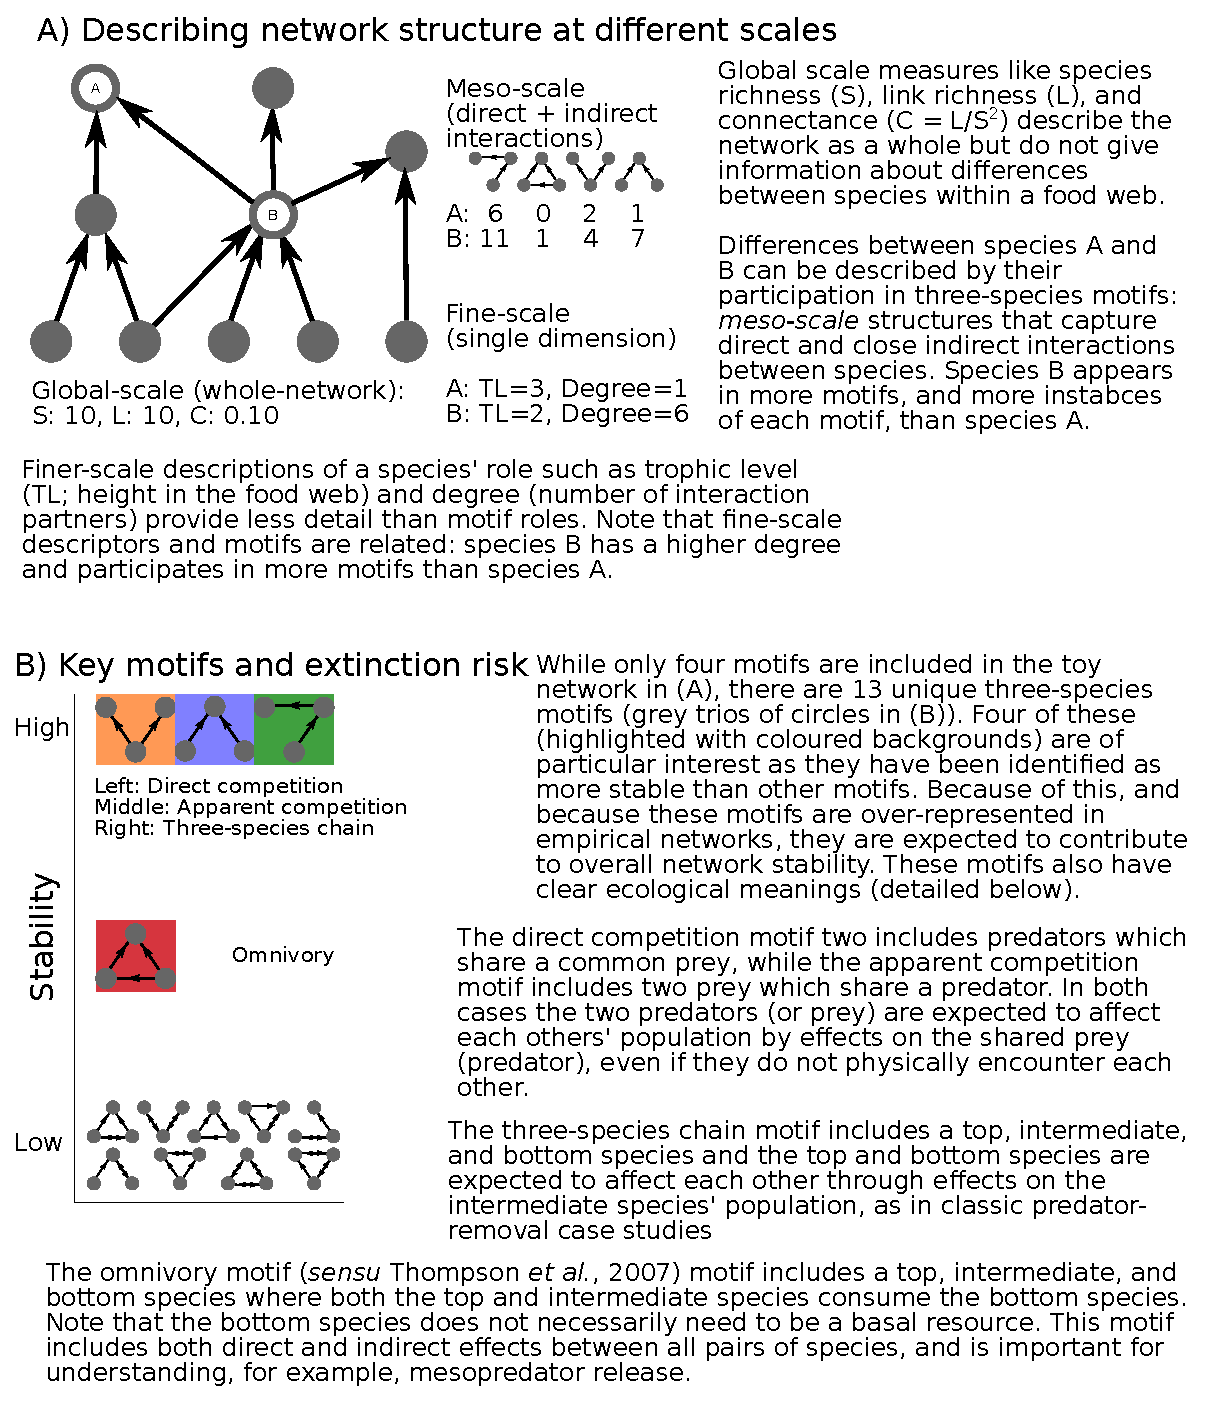
\includegraphics[width=\textwidth]{figures/motifs_box.eps}
        %DIFDELCMD < \caption{%
{%DIFAUXCMD
%DIFDELCMD < \small %%%
\textbf{\DIFdelFL{A}}%DIFAUXCMD
\DIFdelFL{) Food web structure can be described at several different scales. Global scale measures like species richness (S), link richness (L), and connectance (C = L/S$^2$) describe the network as a whole but do not give information on how the extinction risk differs for species within a food web (i.e., species A and B; labelled). Differences between these species can be described by their participation in three-species motifs: }\emph{\DIFdelFL{meso-scale}} %DIFAUXCMD
\DIFdelFL{structures that capture direct and close indirect interactions between species. Here, a species' }\emph{\DIFdelFL{motif role}} %DIFAUXCMD
\DIFdelFL{is a vector describing the number of times it appears in each motif. Only four motifs are included in the toy network shown, indicated by small diagrams to the right. Finer-scale descriptions of a species' role such as trophic level (TL; height in the food web) and degree (number of interaction partners) also capture differences between species but do not provide as much detail as motif roles.}%DIFDELCMD < \\
%DIFDELCMD <         %%%
\textbf{\DIFdelFL{B}}%DIFAUXCMD
\DIFdelFL{) There are 13 unique three-species motifs. Four of these (highlighted with coloured backgrounds and shown in colour in the inset network) are of particular interest. These four motifs have been identified as more stable than other configurations of interacting species and as likely to stabilize the food web as a whole. Moreover, these motifs have clear ecological meanings and have been studied in isolation as well as in food-web contexts.}%DIFDELCMD < \\
%DIFDELCMD <         %%%
\DIFdelFL{The direct competition motif (orange, top left) includes two predators which share a common prey. The predators are expected to affect each other by modulating the prey's population even if they do not physically encounter each other. Similarly, the apparent competition motif (blue, top middle) includes two prey which share a common predator and are expected to affect each other by modulating the predator's population. 
        The three-species chain (green, top right) includes a top, intermediate, and bottom species and the top and bottom species are expected to affect each other through effects on the intermediate species' population. The omnivory motif (}\emph{\DIFdelFL{sensu}} %DIFAUXCMD
\DIFdelFL{Thompson }\emph{\DIFdelFL{et al.}}%DIFAUXCMD
\DIFdelFL{, 2007) motif (red, middle) includes a top, intermediate, and bottom species where both the top and intermediate species consume the bottom species. Note that the bottom species does not necessarily need to be a basal resource. This motif includes both direct and indirect effects between all pairs of species.}}
        %DIFAUXCMD
%DIFDELCMD < \label{motifs}
%DIFDELCMD <     \end{figure}
%DIFDELCMD < 

%DIFDELCMD <   %%%
\DIFdel{Given these early indications that some motifs are more stable than others, we may also expect that a species' role-- here defined as the frequency with which it participates in different motifs --could affect its probability of extinctionfollowing a perturbation.
    Specifically, we expect that species participating more frequently in the stable motifs identified by~}%DIFDELCMD < \citet{Borrelli2015a} %%%
\DIFdel{are less likely to go extinct than species whose roles are dominated by other motifs. Here, we investigate this question }\DIFdelend \DIFaddbegin \DIFadd{Here, we investigate the relationship between species roles and extinction risk }\DIFaddend by simulating the removal of species from simulated networks at stable equilibria. We test 1) whether species' roles are related to their time to extinction following the removal of another species in the network \DIFdelbegin \DIFdel{, }\DIFdelend \DIFaddbegin \DIFadd{and }\DIFaddend 2) \DIFdelbegin \DIFdel{whether participation in particular motifs (especially the stable motifs described above) is correlated }\DIFdelend \DIFaddbegin \DIFadd{if so, which motifs show the strongest correlations }\DIFaddend with time to extinction\DIFdelbegin \DIFdel{, and }\DIFdelend \DIFaddbegin \DIFadd{.
    Because of the non-independence of different network measures, we also test }\DIFaddend 3) whether these correlations are driven by potential relationships between species' participation in various motifs and simpler definitions of species roles (degree, trophic level). \DIFdelbegin \DIFdel{Our overall aim is to establish whether changes in species' roles can, in future, be used to evaluate whether species are at increasing or decreasing risk of extinction}\DIFdelend \DIFaddbegin \DIFadd{Taken together, the results we obtain for these tests show that species are generally consistent in their vulnerability to disturbances, regardless of the location in the network of that disturbance, and this vulnerability is shaped by both motif roles and other network parameters}\DIFaddend .


%DIF <  Approx. 1000 words of introduction
\DIFdelbegin %DIFDELCMD < 

%DIFDELCMD <   %%%
%DIF <  Stability of biological networks has been related to the frequency of different motifs.
  %DIF <  - Prill2005 transcription networks are more stable if they contain more "structurally stable" motifs (motifs whose structures mean a larger parameter space of signs and strengths is stable) motifs. Most stable motifs were apparent competition, direct competition, chain, omnivory (all fully structurally stable - will return to steady state if perturbed without oscillations), then quite a sharp drop before other motifs inc. two-way motifs and one-way loop. Two-way loop was least stable. Stable motifs are more abundant in biological networks. Three classes: I) acyclic graphs (no two-way links), fully stable; II) graphs with one two-way link; III) more complicated circuits (two-way link plus a loop, two two-way links, one-way loop, etc).
  %DIF <  - Stouffer2007 showed chain, omnivory over-represented but both competitions under-represented compared to random in 10/16 empirical webs, competition over-represented and omnivory under in 6/16. Double-loop also over-represented... important to distinguish between abundance and statistical over-abundance of motifs. Motifs in empirical networks consistent with the niche model and not nested-hierarchy. 
  %DIF <  - Stouffer2010 only relevant for pointer to Stouffer2007
  %DIF <  - Stouffer2010b average 95\% of all motifs are chain, omnivory, apparent and direct competition. In isolation, species in tri-trophic chain most likely to all persist, then omnivory, then apparent competition, the direct competition. More species persist in food webs with many chains and omivory, persistence decreases with more apparent and direct competition.
  %DIF <  - Stouffer2005 empirical connectance ranges 0.026-0.315 (25 to 155 trophic species)
  %DIF <  - Stouffer2012 54 distinct roles across 32 webs, up to 22 roles per web (not related to size of web or taxonomic diversity). 46 roles for intermediate species, remainder are basal/int and int/top. Closely related species have similar roles, species with similar roles have similar benefits to their community (based on how much stability increases/decreases when a single motif is added). *Check SI for more details on benefit analysis.
  %DIF <  - Kondoh2008 Intraguild predation modules can be stable if 1) prey is a superior competitor for the resource or 2) extra-module forces such as additional resources exist that benefit the prey more than the predator. In Caribbean food web, all but two species participate in at least 1 IGP module and three sharks are in \>1000. Intrinsically-stable modules were over-represented. Non-intrinsically stable modules were more likely to have external influences favouring prey. If externally-stablised IGP are stabilised by other IGP, may be vulnerable to perturbations. Expect more external stabilisation from internally-stable IGP. This is exactly what was found.
  %DIF <  - Borrelli2015 Systems may be nonadaptively selected for stability by preferential removal of nonstable systems (e.g., culling interactions that lead to oscillations giving low abundances, )
  %DIF <  - Rip2010 Modules that weaken interactions should stabilize the network, looking at "biparallel motif" as one such option - two chains linked at top and bottom. Tested empirically in microcosms, isolated. Generalist consumer de-synchronised its resources, stabilizing community. 
  %DIF <  - Klaise2017 Disagree that the generalized niche model produces networks with similar motif profiles. Clustered food webs with similar profiles using a "hierarchical, agglomerative clustering algorithm based on the Pearson’s correlation coefficient (r)". Distance between webs is sqrt(2*(1-r)). Distances clustered using UPGMA (average linkage) algorithm. Trophic coherence (propensity of species to consume exclusively at the TL below themselves) tunes motif frequencies between two "families", only one of which is generated by the niche model. Main difference is whether omnivory is strongly over- or under-represented.
  %DIF <  - Baiser2015 Local networks resemble regional ones if all trophic groups are sub-sampled with similar frequencies. Not particularly relevant.
  %DIF <  - Monteiro2016  [Haydon1994, May1972, Sterner1997] show that modules are more stable with fewer interactions, small variance in interaction strengths, self-damping processes. Used Jacobian to identify stability of each 3- and 4-species motif, looked at frequencies in empirical networks. AC, DC, chain, and omnivory were all stable (omnivory could also be unstable). More stable motifs appeared more frequen tly. Same for 4-species motifs (4\% were stable). Omnivory ranging stable-unstable can explain contradictory results for omnivory in other studies.
  %DIF <  - Gross2009 High variability in interaction strengths stabilizes small webs, destabilizes large ones. Stability also enhanced by generalist predators (high TL) and very vulnerable intermediate consumers. Used very large suite of simulated networks. No talk of motifs.
  %DIF <  - Dambrot 2017 Having few loops seems to stabilize networks, but we don't know how they come to be un-loopy. Probably trophic coherence again. Not super relevant.
  %DIF <  - Otto2007 Bioenergetic model to explore body-mass ratios and stability of tri-trophic chains. Only particular ratios are stable. Body mass also correlates with degree (+ with number of prey, - with number of predators)
  %DIF <  - Bascompte2005 Ealier work (McCann1998) emphasizes stabilizing role of omnivory but nobody tested whether omnivory over-represented. Apparent competition and intraguild predation (4-sp, two chains with one middle sp. eating the other) more common than expected, omnivory more variable. 
  %DIF <  - Rooney2012 Existence of fast and slow energy channels is stabilizing because it de-synchronises prey populations. Interactions in slow channels also tend to be weaker. Mostly about size and stability.
  %DIF <  - Smith2015 Technical argument about how to standardize community matrices for calculating eigenvalues. Boring (sorry Gyuri)
  %DIF <  - Allesina2008 Pred-prey networks are more likely to be stable than random ones. Varied off-diagonal C from 0.05 to 0.5 with steps of 0.025, size from 10 to 100 with steps of 5. 1000 webs of each size. Determined stability based on percentage of eigenvalues with negative real parts. Did not allow two-way links. Predator-prey networks are more stable than those where signs of interactions are random. Still stable if +/+ and -/- interactions present but less common than pred/prey. Weak interactions not necessary. Short cycles (self-regulation, predator-prey "cycles") may be key, will have greater influence bc. they are smaller. They believe they're supporting the "stable motifs lead to stable networks" lit.
  %DIF <  - Borrelli2014 Food chains are generally 2-4 levels long. When weighted, usually 3 (Ulanowicz2013). Probably not because of inefficient transfer (productivity not strongly correlated with maxTL). Longer food chains take longer to stabilize following a perturbation. Looking at stability of mini-webs and larger random & niche model ones. Found that quasi sign-stability (a la Allesina2008) decreases with increasing chain length, dropping sharply after 3 for mini-webs to almost 0 for length 6.  
  %DIF <  - Borrelli2015 This is the one about motifs and stability. Using Jacobian eigenvalue stability (return to equilibrium following small perturbation). Looked at sign stability of each motif in isolation, Z-scores in empirical webs. Chains, apparent competition, and direct competition were all more likely to be stable and over-represented. Omnivory was moderately likely to be stable, typically under-represented. Could indicate that unstable motifs are more likely to be "pruned", selecting for stability of the whole system. 
  %DIF <  - German thesis Restricted to pairwise interactions and chains.
  %DIF <  - Wootton2016a Pulse vs. press disturbance important. Used press disturbance because many anthropogenic effects thus, many affect one species disproportionately. Affected species may or may not be the one that goes extinct. Tested how web size and connectance affected resistance (size of disturbance required to cause extinction), how traits of disturbed species affected outcome. Found that smaller, less-connected networks were more resistant, focal extinctions more likely. 59\% of extinctions focal, 24\% of extinctions involve indirect interaction partners, 16\% of extinctions predators of focal species, 1\% of extinctions prey of focal species. Higher degree species were more llikely to cause extinction of predators, prey extinctions came from high S, high C webs with focal species with high degree. 
  \DIFdelend

\section*{Methods}
    \subsection*{Generating networks and extinctions}
    	\subsubsection*{Generating food webs}

    		We simulated a suite of food webs based on the probabilistic niche model, which assigns predator-prey links based on the body-mass ratios between \DIFaddbegin \DIFadd{individuals of different }\DIFaddend species~\citep{Williams2000,Delmas2017}. The meso-scale structure of \DIFdelbegin \DIFdel{such }\DIFdelend \DIFaddbegin \DIFadd{niche-model }\DIFaddend networks closely mimics that of empirical food webs~\citep{Stouffer2007}. To \DIFdelbegin \DIFdel{parameterize the model, we specified a predator-prey body-mass ratio of 3.065 based on the estimate for vertebrates (averaged across ecosystem and metabolic types) in~}%DIFDELCMD < \citet{Brose2006}%%%
\DIFdel{. We excluded reported body-mass ratios for invertebrates as these could include parasites and parasitoids, which are generally smaller than their prey, and because interactions among vertebrates are better represented in the food-web literature than interactions involving invertebrates. To }\DIFdelend ensure that we captured a variety of realistic community sizes and structures, we generated networks ranging between 50 and 100 species (in steps of 10) with \DIFdelbegin \DIFdel{connectances }\DIFdelend \DIFaddbegin \DIFadd{connectance values }\DIFaddend between 0.02 and 0.2 (in steps of 0.02). The range of network sizes was chosen to reflect moderately well-sampled empirical webs while working within our computational limits, while the range of \DIFdelbegin \DIFdel{connectances }\DIFdelend \DIFaddbegin \DIFadd{connectance values }\DIFaddend was chosen to cover that observed in \DIFaddbegin \DIFadd{most }\DIFaddend empirical food webs~\DIFdelbegin %DIFDELCMD < \citep{}%%%
\DIFdelend \DIFaddbegin \citep{Dunne2002}\DIFaddend . We generated a total of 100 networks with each combination of parameters, for a total of 6000 networks \DIFaddbegin \DIFadd{(}\emph{\DIFadd{Appendix S1}}\DIFadd{)}\DIFaddend . All networks were \DIFdelbegin \DIFdel{simulated }\DIFdelend \DIFaddbegin \DIFadd{generated }\DIFaddend using the function \DIFdelbegin \DIFdel{"}\DIFdelend \DIFaddbegin \DIFadd{``}\DIFaddend nichemodel" within the Julia language package \emph{BioEnergeticFoodWebs}~\citep{bioenergeticfw,Delmas2017}. If a simulated network contained any disconnected species (species without predators or prey) or disconnected components (a group of species connected amongst themselves but not to the rest of the network), the network was rejected and a new network simulated. Finally, networks where the path lengths between each species and a basal resource could not be resolved \DIFaddbegin \DIFadd{(i.e., trophic levels were undefined) }\DIFaddend were rejected and new networks simulated.

  
    		After \DIFdelbegin \DIFdel{assigning biomasses}\DIFdelend \DIFaddbegin \DIFadd{generating the network structure}\DIFaddend , we simulated community dynamics \DIFdelbegin \DIFdel{in order to obtain an equilibrium community. To ensure that species did not `recover' from unrealistically low biomasses, we considered a species extinct if it dropped below a threshold biomass of 1$\times10^{-5}$ and rejected the network. Community dynamics are based on }\DIFdelend \DIFaddbegin \DIFadd{using the function ``simulate'' from the Julia language package }\emph{\DIFadd{BioEnergeticFoodWebs}}\DIFadd{~}\citep{bioenergeticfw,Delmas2017}\DIFadd{. This function uses }\DIFaddend Lotka-Volterra predator-prey models including density dependence and \DIFdelbegin \DIFdel{with type II }\DIFdelend \DIFaddbegin \DIFadd{type 2 }\DIFaddend functional responses for all species (please see~\citet{Delmas2017} for full details\DIFdelbegin \DIFdel{; all }\DIFdelend \DIFaddbegin \DIFadd{).
    		All }\DIFaddend non-basal species were designated as vertebrates to ensure a good match between metabolic and predator-prey \DIFdelbegin \DIFdel{bodymass ratio values)}\DIFdelend \DIFaddbegin \DIFadd{body-mass ratio values. Metabolic rates in the Lotka-Volterra model are based on each species' body mass (i.e. mass of a single individual). We assigned relative body masses based on each species' trophic level. Trophic levels, in turn, were calculated based on the food-web structure provided by the niche model. Specifically, we use the shortest trophic level (STL), i.e. the shortest path between the species and a basal species~}\citep{Hairston1993}\DIFadd{. After basal species were assigned a body mass of 1, we used a predator-prey body-mass ratio of 3.065 to calculate the relative body masses of higher trophic levels. We selected this ratio based on the estimate for vertebrates (averaged across ecosystem and metabolic types) in~}\citet{Brose2006}\DIFadd{. We excluded reported body-mass ratios for invertebrates as these could include parasites and parasitoids, which are generally smaller than their prey, and because interactions among vertebrates are better represented in the food-web literature than interactions involving invertebrates.
    		}

    		
    		\DIFadd{The persistence of each species in our simulated networks also depends on its population biomass. 
    		We randomly assigned initial population biomasses (i.e. cumulative biomass across all individuals of a species) for each species from a uniform distribution }[\DIFadd{0,1}]\DIFadd{. Note that population biomasses and individual body masses are not calculated on the same scale. We then simulated community dynamics for 1000 time steps to obtain an equilibrium community. We use an equilibrium community to ensure that secondary extinctions are caused by the initial disturbance (i.e. removal of a species) and not due to existing disequilibrium. To ensure that species did not `recover' from unrealistically low biomasses during the simulation, we considered a species extinct if it dropped below an arbitrary threshold biomass of 1$\times10^{-5}$. When simulating initial (ie. pre-perturbation or equilibrium) dynamics, we rejected any network where one or more species dropped below this biomass threshold}\DIFaddend . Consumers were assumed to have no preferences such that the consumption rate $w_{ij}$ of \DIFaddbegin \DIFadd{predator }\DIFaddend $i$ eating \DIFaddbegin \DIFadd{prey }\DIFaddend $j$ is equal to $\frac{1}{n}$, where $n$ is the number of prey for predator $i$. If the network did not reach an equilibrium with all species persisting \DIFdelbegin \DIFdel{after }\DIFdelend \DIFaddbegin \DIFadd{for }\DIFaddend 1000 time steps, a new set of initial population biomasses was applied and the simulation repeated until an equilibrium with all species persisting was obtained.
    		\DIFaddbegin \DIFadd{If a stable equilibrium still had not been reached after 100 sets of randomly-assigned initial biomasses, we discarded the network and simulated another to replace it.
    }\DIFaddend 

    
    	\DIFdelbegin \subsection*{\DIFdel{Calculating motifs and species roles}}
%DIFAUXCMD
\DIFdelend \DIFaddbegin \subsubsection*{\DIFadd{Calculating species roles}}
    \DIFaddend 

    
    		We were interested in whether species' roles at equilibrium are related to their response to a perturbation, in this case the removal of another species in the network. We defined each species' role as the number of times it appears in each unique three-species motif, following~\citet{Stouffer2012,Cirtwill2015}. \DIFdelbegin \DIFdel{As our }\DIFdelend \DIFaddbegin \DIFadd{Note that each set of three interacting species forms exactly one motif~}\citep{Cirtwill2018FoodWebs}\DIFadd{. Our main }\DIFaddend focus is on how different motifs might affect extinction risk, \DIFdelbegin \DIFdel{we do not consider }\DIFdelend \DIFaddbegin \DIFadd{but we also consider how }\DIFaddend the different positions species may take within a motif \DIFaddbegin \DIFadd{could provide extra information on vulnerability to extinction}\DIFaddend . We expect that appearing more frequently in stable motifs (three-species chain, apparent and direct competition, and omnivory) will correlate with lower extinction risk while appearing more frequently in unstable motifs (those containing two- or three-species loops) will be \DIFdelbegin \DIFdel{related to }\DIFdelend \DIFaddbegin \DIFadd{associated with }\DIFaddend higher extinction risk.	Note that cannibalistic links were ignored when calculating motif frequencies within a network and species' roles, although they were included when calculating connectance. As well as these \DIFdelbegin \DIFdel{'}\DIFdelend \DIFaddbegin \DIFadd{`}\DIFaddend raw' motif roles, we calculated \DIFdelbegin \DIFdel{'degree normalized}\DIFdelend \DIFaddbegin \DIFadd{`species-normalised}\DIFaddend ' motif roles for each species by dividing the number of appearances in each motif by the total number of times the species appears in any motif (as in~\citet{Cirtwill2015}\DIFdelbegin \DIFdel{). These 'normalized motifs' should control for differences in species' degrees (numbers of interaction partners}\DIFdelend \DIFaddbegin \DIFadd{; this total is expected to strongly correlate with degree}\DIFaddend ). Finally, we also calculated \DIFdelbegin \DIFdel{'network normalized}\DIFdelend \DIFaddbegin \DIFadd{`network-normalised}\DIFaddend ' motif roles, defined as the \DIFdelbegin \DIFdel{z-score }\DIFdelend \DIFaddbegin \DIFadd{$Z$-score }\DIFaddend of the number of times a focal species appears in each motif compared to the number of times all species in the network appear in the focal motif.
    		The \DIFdelbegin \DIFdel{degree }\DIFdelend \DIFaddbegin \DIFadd{species }\DIFaddend normalisation allows us to test whether trends in stability with motif participation are due to differences in \DIFdelbegin \DIFdel{species' degrees}\DIFdelend \DIFaddbegin \DIFadd{the total number of motifs a species appears in}\DIFaddend , while the network normalisation allows us to test whether trends in stability \DIFdelbegin \DIFdel{with participation in different motifs }\DIFdelend are related to how unusual \DIFdelbegin \DIFdel{each speciesis within its communitycontext}\DIFdelend \DIFaddbegin \DIFadd{a species' motif participation is relative to other species in its community, rather than which specific motifs a species participates in}\DIFaddend .

    	%DIF <  Apart from motif-based measures of species' positions in their communities, we calculated their degrees and short-weighted trophic levels. Degree is simply the number of interaction partners for each species. A species' short-weighted trophic level is the mean of its shortest trophic level an prey-averaged trophic level. The shortest trophic level is calculated based on the length of the shortest food chain between the focal species and any basal resource. Basal resources are assigned a trophic level of one and other species are assigned a shortest trophic level of one plus the trophic level of their prey. Prey-averaged trophic level is calculated based on the set of all shortest food chains between the focal species and any basal resources. The focal species' prey-averaged trophic level is the mean trophic level of its prey plus one. These alternative topological measures will be used to evaluate how strongly species' motif roles are related to their response to perturbation compared to other measures of position within a network. These measures were used to test how consistent motif roles and motif participation are for species which share the same degree or trophic level. [[Need to add this formally once I do it.]]
\DIFdelbegin %DIFDELCMD < 

%DIFDELCMD <   %%%
\subsection*{\DIFdel{Perturbing networks}}
%DIFAUXCMD
\DIFdelend \DIFaddbegin \subsubsection*{\DIFadd{Perturbing networks}}
    \DIFaddend 

    		After identifying species' roles in the equilibrium networks, we perturbed the networks by removing a single species. After this removal, community dynamics were simulated for 50 rounds of 10 time-steps (500 time-steps total). After each round, any species with a biomass below our threshold of 1$\times10^{-5}$ was considered to have gone extinct and its biomass was set to 0. We recorded the biomass of each species after each round, as well as the round in which any additional extinctions occurred. After 500 time-steps, we reset the network to its original state (including all species). We then removed a new species and again simulated community dynamics. We repeated this process until all species had served as the initial removal.
    		We then calculated the mean time to extinction across all removals as an overall measure of each species' vulnerability (\emph{Appendix \DIFdelbegin \DIFdel{SQ}%DIFDELCMD < }%%%
\DIFdel{, Supplemental Information). 
    		}\DIFdelend \DIFaddbegin \DIFadd{S2}}\DIFadd{). 
    		Species which did not go extinct in a given simulation were assigned an extinction time of 500.
    		}\DIFaddend Time to extinction was highly correlated across removals in all combinations of S and C, indicating that this is a robust measure.


	\subsection*{\DIFdelbegin \DIFdel{Testing effects of species' roles on time to extinction}\DIFdelend \DIFaddbegin \DIFadd{Statistical Analysis}\DIFaddend }

        \subsubsection*{\DIFdelbegin \DIFdel{Relating overall }\DIFdelend \DIFaddbegin \DIFadd{Is }\DIFaddend motif \DIFdelbegin \DIFdel{roles to time }\DIFdelend \DIFaddbegin \DIFadd{participation related }\DIFaddend to \DIFdelbegin \DIFdel{extinction}\DIFdelend \DIFaddbegin \DIFadd{persistence?}\DIFaddend }

            \DIFdelbegin \DIFdel{To test for a relationship between persistence and species' overall roles, we therefore }\DIFdelend \DIFaddbegin \DIFadd{We are interested in whether the set of motifs in which a species appears at `equilibrium' is related to its persistence (here defined as time to extinction following the removal of another species). 
            To address this question, we can consider the motif participation role as a whole or the relationships between participation in each motif and persistence. 
            The first approach provides a more holistic view of the relationship between meso-scale structure and extinction risk, while the second may identify specific meso-scale structures with especially strong relationships to persistence.
}


            \textbf{\DIFadd{Motif participation as a whole}}

                \DIFadd{To test whether motif participation as a whole is related to persistence, we }\DIFaddend fit a series of PERMANOVAs relating \DIFdelbegin \DIFdel{dissimilarity in roles to differences in mean time to extinction.
      PERMANOVA is a multivariate analogue of classic ANOVA which, importantly, does not assume that response data are normally distributed~}%DIFDELCMD < \citep{Anderson2001}%%%
\DIFdel{. 
                To avoid effects of network size and connectance on time to extinction}\DIFdelend \DIFaddbegin \DIFadd{the Bray-Curtis dissimilarity in species' motif participation vectors to their persistence times (see }\emph{\DIFadd{Appendix S3}} \DIFadd{for details). 
                Due to computational constraints}\DIFaddend , we fit \DIFdelbegin \DIFdel{separate PERMANOVAs for each }\DIFdelend \DIFaddbegin \DIFadd{one PERMANOVA per }\DIFaddend combination of network size and connectance (60 \DIFdelbegin \DIFdel{PERMANOVAs in total). 
                As conducting so many tests risks obtaining significant results by chance, we applied the correlated Bonferroni correction~}%DIFDELCMD < \citep{Drezner2016} %%%
\DIFdel{before evaluating significance.
      We calculated Bray-Curtis dissimilarity in the counts of each motif in the role of each species~}%DIFDELCMD < \citep{Baker2015,Cirtwill2015} %%%
\DIFdel{and related these dissimilarities to differences in mean time to extinction.
                We fit all PERMANVOAs using the R~}%DIFDELCMD < \citep{R} %%%
\DIFdel{function 'adonis' from the package }\emph{\DIFdel{vegan}}%DIFAUXCMD
\DIFdel{~}%DIFDELCMD < \citep{vegan} %%%
\DIFdel{and calculated $p$-values using 9999 unstratified permutations.
            To support these PERMANOVAs, we fit a linear model testing whether the raw frequencies of each motif }\DIFdelend \DIFaddbegin \DIFadd{combinations). 
                We repeated these sets of PERMANOVAs for each version of motif participation vectors (counts, species-normalised, and network-normalised; 180 PERMANOVAs in total).
                Because the assumption of equal varibility that underlies a PERMANOVA test was not met (see }\emph{\DIFadd{Appendix S4}}\DIFadd{), the results of these tests are indicative but not conclusive.
                Further, because of this violation of assumptions, we did not use PERMANOVAs to test whether motif roles including positions }\DIFaddend were related to \DIFdelbegin \DIFdel{mean }\DIFdelend time to extinction\DIFdelbegin \DIFdel{(}\emph{\DIFdel{Appendix SX}}%DIFAUXCMD
\DIFdel{, Supplemental Information)}\DIFdelend .


            \DIFdelbegin \subsubsection*{\DIFdel{Identifying the motifs most strongly related to time to extinction}}
%DIFAUXCMD
\DIFdelend \DIFaddbegin \textbf{\DIFadd{Participation in particular motifs}}
\DIFaddend 

                \DIFdelbegin \DIFdel{While the PERMANOVA can tell us whether a species' role as a whole is related to its mean time to extinction, it does not reveal which motifs have the strongest effect on time to extinction.
                To answer this question, we used a partial least squares (PLS) regression to identify combinations of motifs which, together, explain substantial variation in time to extinction. 
      Similar to a principal components analysis (PCA) , PLS involves projecting the observed variables (in this case, participation in different motifs ) into a new space and identifying latent variables made up of linear combinations of the observed variables~}%DIFDELCMD < \citep{Mevik2007}%%%
\DIFdel{. 
                In our case, these latent variables represent combinations of motifs which, together, explain substantial variation in persistence.
As well as simply identifying key motifs, we were interested in understanding whether species achieve longer mean times to extinction because their roles contain greater proportions of certain motifs or because they participate in certain motifs more than other species within the same network.
      }\DIFdelend \DIFaddbegin \DIFadd{For a more detailed perspective on relationships between motif participation and persistence, we fit linear mixed-effect models including the effect of each motif separately.
                Since the motifs containing loops (two-way interactions or three-species loops) are rare in both empirical systems~}\citep{Stouffer2007} \DIFadd{and our simulated networks (means 8.99$\times10^{-4}$-2.06\%) and are all unstable when modelled in isolation~}\citep{Borrelli2015a}\DIFadd{, we pool these loop-containing motifs into an `other' group (see }\emph{\DIFadd{Appendix S5}} \DIFadd{for details about how each version of motifs were pooled). 
                We considered each stable motif (apparent competition, direct competition, omnivory, and three-species chain) individually.
}\DIFaddend 


                \DIFdelbegin \DIFdel{To distinguish between these two possibilities}\DIFdelend \DIFaddbegin \DIFadd{For each version of motif participation (count, frequency, or $Z$-score)}\DIFaddend , we fit \DIFdelbegin \DIFdel{two separate PLS regressions.
      In the first, we used }\DIFdelend \DIFaddbegin \DIFadd{a  linear mixed-effect model (LMM) of the form:
}

                \begin{equation}
                    \DIFadd{\tau_{in} \approx \alpha_{i} + \delta_{i} + o_{i} + \chi_{i} + \omega_{i} + S_{n}:C_{n} +N_n,
                    \label{eq:persistence_motifs}
                }\end{equation}

                \DIFadd{where $\tau_{in}$ is the }\DIFaddend mean time to extinction \DIFdelbegin \DIFdel{as the response and network size, connectance, the interaction between size and connectance, in-degree (number of prey) , shortest trophic level, and degree-normalized motif participation as predictors.
      We include network parameters and other measures of species degrees as these may affect the motif roles available to each focal species.
      In the second,  we used the same variables except for network-normalized motif participation (i.e., $Z$-scores of participation).
      The first regression tests whether a species' absolute participation in different motifs affects its time to extinction (e.g., whether participating in more }\DIFdelend \DIFaddbegin \DIFadd{(persistence) of species $i$ belonging to network $n$,  $\alpha_{i}$, $\delta_{i}$, $o_{i}$, and $\chi_{i}$ are the species' participation in the apparent competition, direct competition, omnivory, and }\DIFaddend three-species \DIFdelbegin \DIFdel{chains leads to longer persistence).
      The second tests whether a }\DIFdelend \DIFaddbegin \DIFadd{chain motifs (respectively), $\omega_{i}$ is the }\DIFaddend species' participation in \DIFdelbegin \DIFdel{more or fewer of different motifs, relative to otherspecies in the }\DIFdelend \DIFaddbegin \DIFadd{the unstable/`other' motif group, $S_{n}:C_{n}$ is a random effect of the size and connectance of network $n$, and $N_n$ is a random effect of belonging to }\DIFaddend network \DIFdelbegin \DIFdel{, affects its time to extinction.
                }%DIFDELCMD < 

%DIFDELCMD <       
%DIFDELCMD <       %%%
\DIFdel{In order to test the predictive ability of both models, we initially fit them on the first 50 networks of each size and connectance combination, reserving the remaining 50 networksas test data. 
                To prevent the non-motif predictors from exerting overly large influence on the models, we centred and scaled these predictors.
                This ensured similar ranges between normalised motifs and the other predictors}\DIFdelend \DIFaddbegin \DIFadd{$n$.
                The random effect of global network structure controls for differences in mean persistence between, for example, highly-connected and weakly-connected networks. 
                The random effect of network ID controls for the fact that all species in the same network have the same pool of motifs to participate in and are therefore non-independent.
                These models indicate whether each motif is positively or negatively correlated with persistence time, and how much variation in persistence time can be explained by each version of motif participation}\DIFaddend . 
                We fit \DIFdelbegin \DIFdel{both regressions }\DIFdelend \DIFaddbegin \DIFadd{the LMMs }\DIFaddend using the R~\citep{R} function \DIFdelbegin \DIFdel{'plsr}\DIFdelend \DIFaddbegin \DIFadd{`lmer}\DIFaddend ' from the package \emph{\DIFdelbegin \DIFdel{pls}\DIFdelend \DIFaddbegin \DIFadd{lmerTest}\DIFaddend }~\DIFdelbegin %DIFDELCMD < \citep{pls} %%%
\DIFdel{and cross-validated the regressions using 10 randomly-selected segments of the data and re-fitting.This cross-validation allows us to select the optimum number of components to include in the regression.
                We selected the optimum model as the one with the fewest components with an mean squared error of prediction (MSEP) less than one standard deviation away from the best model. 
                MSEP is a measure of the error obtained when re-fitting a PLS or PCA model on test data, and is commonly used to select the optimum number of components~}%DIFDELCMD < \citep{Mevik2004}%%%
\DIFdel{)Model selection was performed using the R~}%DIFDELCMD < \citep{R} %%%
\DIFdel{function 'selectNcomp' from the package }\emph{\DIFdel{plsr}}%DIFAUXCMD
\DIFdel{~}%DIFDELCMD < \citep{pls} %%%
\DIFdel{using the method 'onesigma'.
                After selecting the optimum number of components for each model, we re-fit the PLS regression including only the selected components. 
      We then summed the coefficients of each predictor across axes to obtain an overall measure of }\DIFdelend \DIFaddbegin \citep{lmerTest} \DIFadd{and calculated variance explained using }\DIFaddend the \DIFdelbegin \DIFdel{effect of each predictor on mean time to extinction.
}\DIFdelend \DIFaddbegin \DIFadd{function `r.squaredGLMM' from the package }\emph{\DIFadd{MuMIn}}\DIFadd{~}\citep{MuMIn}\DIFadd{.
                }\DIFaddend 

                
                \DIFdelbegin \subsubsection*{\DIFdel{Relating motif roles to other role definitions}}
    %DIFAUXCMD
\DIFdelend \DIFaddbegin \DIFadd{Note that, in the species-normalised motif participation vectors, the frequencies of all motifs must sum to 1 and are therefore not independent. 
                Participation in the count and $Z$-score motifs also may not be independent (e.g., species which participate in especially many interactions may have high counts and $Z$-scores of several motifs).
                To illustrate these potential interdependences, we also present the correlations among all motifs for each version of motif participation, calculated using the function `lmer' as above.
                }\DIFaddend 

                
                \DIFdelbegin \DIFdel{Finally, we wanted to test the possibility that the relationships we observe between motif roles and time to extinction might be due to underlying relationships between species' numbers of interaction partners (degree) and their roles.
      Species with more interaction partners will participate in more motifs (as each combination of three interacting species represents a unique motif).These species might also participate in a more diverse set of motifs, or might have roles in which certain motifs are over-represented.
                To test these possibilities, we tested for relationships between a species degree and both the count and proportion of each motif in }\DIFdelend \DIFaddbegin \DIFadd{To obtain more detail about the relationships between motif participation and persistence time, we repeated the analyses above while defining roles based on a species' participation in each unique position (e.g., top, middle, and bottom species in a three-species chain) in each motif.
                As we are most interested in relationships between persistence and }\DIFaddend the \DIFdelbegin \DIFdel{species' role using }\DIFdelend \DIFaddbegin \DIFadd{apparent competition, direct competition, omnivory, and chain motifs, we grouped all  positions in other motifs into an `other' category, similar to the way we pooled `other' motifs above.
                We calculated raw count, species-normalised, and network-normalised roles including positions as above.
                }


        \subsubsection*{\DIFadd{Adding context: how does motif participation relate to simple roles?}}

            \DIFadd{To interpret the results of the analyses above, especially the LMMs, we must bear in mind the potential for motif participation to reflect differences in degree, trophic level, and global network structure. 
            To establish this context, we therefore fit }\DIFaddend a series of linear \DIFdelbegin \DIFdel{regressions (26 regressions total) .
      All regressions included degreeas a predictor and the count or proportion of the focal motif as a response and were fit with the R~}%DIFDELCMD < \citep{R} %%%
\DIFdel{base function 'lm' .
      Because species with no interaction partners (zero degree) would necessarily have no motif roles, we enforced an intercept of zero}\DIFdelend \DIFaddbegin \DIFadd{models (LMs) relating degree, trophic level, network size, and connectance to each version of the motif role (}\emph{\DIFadd{Appendix S6}}\DIFadd{). 
            These LMs also included a random effect of global network structure.
            For ease of interpretation, we once again grouped the loop-containing motifs into an `other' group. 
            When using species-normalised motifs, we removed the `other' motifs from the model to avoid a rank-deficient model matrix}\DIFaddend .
            As with \DIFdelbegin \DIFdel{our PERMANOVA analysis, fitting so many regressions runs the risk of obtaining significant results by chance.
            To increase the likelihood of detecting a true relationship between species' degrees and motif roles, we applied the correlated Bonferroni correction~}%DIFDELCMD < \citep{Drezner2016} %%%
\DIFdel{before evaluating significance of these regressions }\DIFdelend \DIFaddbegin \DIFadd{the relationship between motif participation and persistence time, we repeated the analyses above for roles including positions within each of our focal motifs.
            }

            
            \DIFadd{To complete this background, we fit a regression of persistence against degree, trophic level, and their interaction, as well as a random effect of global network structure (}\emph{\DIFadd{Appendix S7}}\DIFadd{). 
            These regressions are intended only to confirm whether our simulations show the expected increase in persistence with degree and decrease in persistence with trophic level}\DIFaddend . 


\section*{Results}
    \subsection*{\DIFdelbegin \DIFdel{Relating overall motif roles to mean time }\DIFdelend \DIFaddbegin \DIFadd{Motif participation was related }\DIFaddend to \DIFdelbegin \DIFdel{extinction}\DIFdelend \DIFaddbegin \DIFadd{persistence}\DIFaddend }

		\DIFdelbegin \DIFdel{Species' roles }\DIFdelend \DIFaddbegin \DIFadd{Our series of PERMANOVA tests demonstrated that species' overall motif roles (raw, species-normalised, and network-normalised) }\DIFaddend were correlated with their mean time to extinction across all combinations of species richness and connectance (\DIFdelbegin \DIFdel{Table~\ref{permtable}}\DIFdelend \DIFaddbegin \DIFadd{Fig. }\emph{\DIFadd{S1}}\DIFadd{, Tables }\emph{\DIFadd{TS1-S3, Appendix S3}}\DIFaddend ). 
        Taken individually, each PERMANOVA was significant (all $p$\textless0.025). Moreover, after applying the correlated Bonferroni correction~\citep{Drezner2016}, all PERMANOVAs remained significant.
		\DIFdelbegin \DIFdel{While values of the pseudo-$F$ statistic increased steadily with increasing species richness, $p$-values were similar across values }\DIFdelend \DIFaddbegin \DIFadd{However, some of these significant results are likely false positives since the variability of raw motif roles was not consistent across mean times to extinction for most combinations }\DIFaddend of species richness and connectance (\DIFdelbegin \DIFdel{Fig.~\ref{permfig}). 
        Neither the pseudo-$F$ nor the $p$-values demonstrate an obvious interaction between species richness and connectance.
        The frequencies of all motifs were significantly related to mean time to extinction, with motifs S1 and S4 having the largest positive associations with time to extinction after taking the observed numbers of each motif into account (}\DIFdelend \DIFaddbegin \DIFadd{Tables }\emph{\DIFadd{S4-6, Appendix S4}}\DIFadd{). 
        In most cases, motif roles were more variable among species with longer times to extinction (Fig. S3,}\DIFaddend Appendix \DIFdelbegin \DIFdel{SX}%DIFDELCMD < }%%%
\DIFdel{, Supplemental Information).
        }%DIFDELCMD < 

%DIFDELCMD <       \begin{figure}[hb!]
%DIFDELCMD <         %%%
%DIFDELCMD < \caption{%
{%DIFAUXCMD
\DIFdelFL{Here we show (}\textbf{\DIFdelFL{A}}%DIFAUXCMD
\DIFdelFL{) the pseudo-$F$ statistics and (}\textbf{\DIFdelFL{B}}%DIFAUXCMD
\DIFdelFL{) the $p$-values for each PERMANOVA relating species' roles to their mean extinction order when all species in the web are separately removed. We fit one PERMANOVA per combination of species richness and connectance. $p$-values for each PERMANOVA are based on 9999 permutations, stratified by network. Symbols below the dotted line in }\textbf{\DIFdelFL{B}} %DIFAUXCMD
\DIFdelFL{indicate a significant $p$-values.}}
        %DIFAUXCMD
%DIFDELCMD < \label{permfig}
%DIFDELCMD <         \includegraphics[height=.5\textheight]{figures/extinction_order/permanova_summary_paper_full.eps}
%DIFDELCMD <         \end{figure}
%DIFDELCMD < 

%DIFDELCMD <   %%%
\subsection*{\DIFdel{Identifying the motifs most strongly related to mean time to extinction}}
%DIFAUXCMD
\DIFdelend \DIFaddbegin \DIFadd{S4).
        This unequal variability means that the PERMANOVA results, while indicative, cannot be taken as conclusive proof that motif roles are related to species' time to extinction.
    }\DIFaddend 


    \DIFdelbegin \DIFdel{After testing whether species' motif roles overall were related to mean times to extinction, we used PLS regressions to identify the motifs which were most strongly associated with persistence.
    }\DIFdelend \DIFaddbegin \subsection*{\DIFadd{Participation in stable motifs was related to persistence}}

        \DIFadd{When defining participation based on counts, increased participation in any stable motif except for omnivory was correlated with longer persistence following species removal (Fig. }\emph{\DIFadd{S9}} \DIFadd{and Table }\emph{\DIFadd{S12, Appendix S8}}\DIFadd{).
        Regressions against motif participation explained only 5.8\% of variation in persistence time (fixed effects only).
        }\DIFaddend When \DIFdelbegin \DIFdel{using the raw (un-normalized) frequencies of motifs, the optimum model 
        }%DIFDELCMD < 

%DIFDELCMD <         
%DIFDELCMD <         %%%
\DIFdel{To determine whether the key motifs differ when considering the shape of a species ' role (i.e. , degree normalization)or how a focal species compares to other in the same network (i.e., network normalization), we used partial least squares regressions with two different normalizations of species roles.
        When normalizing motif }\DIFdelend \DIFaddbegin \DIFadd{defining }\DIFaddend roles based on \DIFdelbegin \DIFdel{degree,  the optimum model included 11 components.
    The first component explained 22.1\% of variation in mean }\DIFdelend \DIFaddbegin \DIFadd{positions within each motif,  increased participation in any of the positions in the omnivory motif was correlated with shorter }\DIFaddend time to extinction \DIFdelbegin \DIFdel{, with the remaining ten components explaining an additional 1\% or less.Taking the 11 components together, the proportion of a species' role made up by motifsD2 and S2 }\DIFdelend \DIFaddbegin \DIFadd{while increased participation in any position in the apparent competition, direct competition, and three-species chain motifs was associated with longer persistence (Fig.~\ref{fig:persistence_positions}, Table }\emph{\DIFadd{S14, Appendix S8}}\DIFadd{).
        Roles including positions explained the same amount of variation in persistence time as roles including whole motifs.
        }

        
        \DIFadd{When defining participation based on frequencies, greater participation in the omnivory, three-species chain, and apparent competition motifs was correlated with longer persistence, while the frequency of the direct competition motif was not significantly associated with persistence }\DIFaddend (Fig. \DIFdelbegin \DIFdel{~\ref{motifs}), trophic level, and the proportion of a species' role made up by motifs D4 and D1 all had large negative effects on mean time to extinction (i.e. 
        species in these roles or with higher trophic levels went extinct faster) (Fig.~\ref{coefficient_sum}A).
        The proportion of a species' role made up by motifs S5, S1, and D2, as well as degree had substantial but smaller positive effects on mean time to extinction.
}\DIFdelend \DIFaddbegin \emph{\DIFadd{S9}} \DIFadd{and, Table }\emph{\DIFadd{S16, Appendix S8}}\DIFadd{).
        However, the amount of variance in persistence time explained by frequencies was extremely low (0.5\%; fixed effects only). 
        The amount of variance in persistence time explained by roles including motif positions was substantially higher (8.1\%; fixed effects only).
        Persistence time increased with the frequency of appearing in the bottom position in the apparent competition motif, the top position of the direct competition motif, and the middle position of the three-species chain motif (Fig.~\ref{fig:persistence_positions}, Table }\emph{\DIFadd{S18, Appendix S8}}\DIFadd{).
}\DIFaddend 

        
        \DIFdelbegin \DIFdel{When normalizing motif roles based on the network (i.e.}\DIFdelend \DIFaddbegin \DIFadd{When defining participation based on $Z$-scores}\DIFaddend , \DIFdelbegin \DIFdel{defining motif participation as }\DIFdelend \DIFaddbegin \DIFadd{unusually high participation in the omnivory motif was associated with shorter persistence while unusually high participation in any other motif was associated with longer persistence (Fig. }\emph{\DIFadd{S9}}\DIFadd{, Table }\emph{\DIFadd{S20, Appendix S8}}\DIFadd{).
        The amount of variance in persistence explained by trends in $Z$-score participation was lower than that explained by counts but higher than that explained by frequencies (2.2\%; fixed effects only).
        The amount of variance in persistence explained by }\DIFaddend $Z$-scores \DIFdelbegin \DIFdel{), the optimum model included four components. Together, however, these four components explained only 14.8\%of variation in mean time to extinction (13.1\%, 1.0\%, 0.6\%, and 0.1\%respectively).
        Taking the four components together, trophic level had a large negative effect on mean time to extinction }\DIFdelend \DIFaddbegin \DIFadd{of appearing in different positions was higher than that explained by participation in whole motifs (4.9\%; fixed effects only).
        Unusually high participation in the bottom position in the apparent competition motif, either position in the direct competition motif, and middle position in the three-species chain were associated with longer persistence }\DIFaddend (Fig.~\DIFdelbegin \DIFdel{\ref{coefficient_sum}B).
    Connectance and over-representation of motif D4 had smaller negative effects on mean time to extinction, while over-representation of motifs S1, S4, S5, and D1 had smaller positive effects on mean time to extinction}\DIFdelend \DIFaddbegin \DIFadd{\ref{fig:persistence_positions}, Table }\emph{\DIFadd{S22, Appendix S8}}\DIFadd{)}\DIFaddend .


    \DIFdelbegin %DIFDELCMD < \begin{figure}[hb!]
%DIFDELCMD <       %%%
%DIFDELCMD < \caption{%
{%DIFAUXCMD
\DIFdelFL{Sum of loadings of normalized motif roles, degree, shortest trophic level (STL), web size (S), connectance (C), and their interaction (S:C) in the optimum number of axes in partial least squares regressions of mean time to extinction against all of the above predictors. We fit separate models for degree normalization (i.e., dividing counts of each motif by the total number of all motifs for the focal species) and network normalization (i.e., calculating $Z$-scores for each motif compared to all species in the network). Stable motifs are shaded in light blue.}}
      %DIFAUXCMD
%DIFDELCMD < \label{coefficient_sum}
%DIFDELCMD <       \includegraphics[height=0.5\textheight]{figures/PLS/total_coefficients.eps}
%DIFDELCMD <       \end{figure}
%DIFDELCMD < 

%DIFDELCMD <   %%%
\DIFdelend \subsection*{\DIFdelbegin \DIFdel{Relating motif roles }\DIFdelend \DIFaddbegin \DIFadd{Motif participation was related }\DIFaddend to \DIFdelbegin \DIFdel{degree}\DIFdelend \DIFaddbegin \DIFadd{simpler roles}\DIFaddend }    

        As expected, \DIFdelbegin \DIFdel{the count of all motifs increased significantly with increasing degree }%DIFDELCMD < [[%%%
\DIFdel{add a table if interesting}%DIFDELCMD < ]]%%%
\DIFdel{.
    The frequency of the four stable motifs (S1, S2, S4, and S5)increased most rapidly with increasing degree }\DIFdelend \DIFaddbegin \DIFadd{a higher degree was associated with higher counts and higher $Z$-scores of any motif (Fig. }\emph{\DIFadd{S5}}\DIFadd{, Appendix }\emph{\DIFadd{S6}}\DIFadd{).
        A higher degree was also associated with higher counts of all positions and higher $Z$-scores of all positions except for the bottom and middle positions of the three-species chain }\DIFaddend (Fig. \DIFdelbegin \DIFdel{~\ref{motif_vs_degree}A).
        Moreover, the proportion of a species' role which is made up by the four stable motifs also increased more rapidly with degree }\DIFdelend \DIFaddbegin \emph{\DIFadd{S6, Appendix S6}}\DIFadd{).
        A higher frequency of omnivory was also associated with higher degree, while the converse was true for all other motifs.
        A higher frequency of any position in the omnivory motif was likewise associated with higher degree, as were higher frequencies of both positions in the apparent competition motif and top positions in the direct competition and three-species chain motifs }\DIFaddend (Fig.~\DIFdelbegin \DIFdel{\ref{motif_vs_degree}B).
        The one-way loop motif }\DIFdelend \DIFaddbegin \DIFadd{\ref{fig:positions_deg}).
        Raw motif participation explained almost all variance in degree, while the correlation between network-normalised ($Z$-score) motif participation and degree was weaker.
        Based on these correlations, raw motif participation provides mostly the same information given by degree while species-normalised }\DIFaddend and \DIFdelbegin \DIFdel{two-way motifs showed weak, although still significant, relationships with degree.
}%DIFDELCMD < 

%DIFDELCMD <     \begin{figure}[hb!]
%DIFDELCMD <       %%%
%DIFDELCMD < \caption{%
{%DIFAUXCMD
\DIFdelFL{As a species has more interaction partners, it participates in more motifs. }\textbf{\DIFdelFL{A)}} %DIFAUXCMD
\DIFdelFL{The counts of the four stable motifs (S1, S2, S4, and S5) in a species' role increased most strongly with increasing degree. }\textbf{\DIFdelFL{B)}} %DIFAUXCMD
\DIFdelFL{The proportion of a species' role made up by the four stable motifs also increased strongly with degree. In both panels, motifs are plotted in order of the strength of their relationship with degree and all relationships were significant. 95\% confidence intervals about the regression lines are too small to be visible in the current plot. In both panels, the four stable motifs are indicated by blue lines while unstable motifs are indicated by yellow lines.}}
      %DIFAUXCMD
%DIFDELCMD < \label{motif_vs_degree}
%DIFDELCMD <       \includegraphics[width=.75\textwidth]{figures/roles/motif_vs_degree.eps}
%DIFDELCMD <       \end{figure}
%DIFDELCMD < 

%DIFDELCMD < %%%
\DIFdel{The relationships between trophic level and participating in different motifs or positions were extremely weak for all versions of motif participation (\emph{Appendix S6}).
        While there were some significant relationships, these trends explain so little variation in trophic level that motif participation and trophic level are likely to convey almost entirely different information about a species' place in the network.
    }\DIFdelend 


\DIFaddbegin \subsection*{\DIFadd{Persistence was related to simpler roles}}
    \DIFaddend 

        \DIFdelbegin \DIFdel{Time to extinction was quite consistent across removals.
        We found that these mean times to extinction were related to species' motif roles.
        While participation in stable motifs was generally associated with }\DIFdelend \DIFaddbegin \DIFadd{Simple roles (degree and trophic level) together explained a moderate amount of variation in persistence ($R^2_m$=0.211, $R^2_c$=0.232).
        Species with higher degrees and lower trophic levels tended to have }\DIFaddend longer mean times to extinction \DIFdelbegin \DIFdel{, the set of motifs that was most strongly associated with mean time to extinction varied depending on the normalization used}\DIFdelend \DIFaddbegin \DIFadd{(}\emph{\DIFadd{Appendix S7}}\DIFadd{).
        However, a negative interaction term means that an increase in degree is less beneficial for species with high trophic level (Fig.~\ref{fig:persistence_degTL}).
    }

    
\section*{\DIFadd{Discussion}}

    \DIFadd{We found that times to extinction were tightly correlated across removals}\DIFaddend . 
    This suggests that \DIFdelbegin \DIFdel{a }\DIFdelend \DIFaddbegin \DIFadd{the position of a focal species within a network can affect its risk of extinction following a disturbance regardless of where in the network the disturbance is applied. 
    This result also justifies our use of mean times to extinction across removals as a measure of a }\DIFaddend species\DIFdelbegin \DIFdel{' time to extinction after a perturbation depends on both participating in more/less of a given motif than other species in the focal network and the extent to which a focal species' role is dominated by different motifs.
    Interpreting the relationships between species roles and persistence is complicated by the relationship between degree and motif participation.
    The count of stable motifs in a species' role tended to increase rapidly with increasing number of interaction partners, indicating that degree may capture similar information about extinctionrisk as more complex measures of species roles}\DIFdelend \DIFaddbegin \DIFadd{' overall risk.
    }

    
    \DIFadd{Taken together, our results show that motif roles are related to mean times to extinction.
    Species-normalised (frequency) motif roles including participation in different positions explained the most variation in time to extinction.
    As expected, participation in positions in the apparent competition, direct competition, and three-species chain were especially associated with longer times to extinction}\DIFaddend .


 	\subsection*{\DIFdelbegin \DIFdel{High consistency of times }\DIFdelend \DIFaddbegin \DIFadd{Times }\DIFaddend to extinction \DIFaddbegin \DIFadd{are highly consistent}\DIFaddend }

		\DIFdelbegin \DIFdel{Species}\DIFdelend \DIFaddbegin \DIFadd{The consistency of species}\DIFaddend ' times to extinction \DIFdelbegin \DIFdel{were tightly correlated across removals . 
    This suggests that species' positions }\DIFdelend \DIFaddbegin \DIFadd{across removals in our simulations suggests that some species are more likely to go extinct than others due to their position }\DIFaddend within a network\DIFdelbegin \DIFdel{influence their extinction risk, regardless of the identity of the removed species and }\DIFdelend \DIFaddbegin \DIFadd{.
        This }\DIFaddend complements other work identifying sets of species which are more vulnerable to extinction due to their traits~\citep{Curtsdotter2011,Ryser2019}. 
		\DIFdelbegin \DIFdel{Earlier work suggests that network properties (}\DIFdelend \DIFaddbegin \DIFadd{Since the }\DIFaddend trophic level and degree \DIFdelbegin \DIFdel{) }\DIFdelend of the species being removed \DIFdelbegin \DIFdel{are also important in determining the location and rate of resulting secondary extinctions}\DIFdelend \DIFaddbegin \DIFadd{can also affect which species, if any, go secondarily extinct}\DIFaddend ~\citep{Wootton2016a,Dunne2002}\DIFdelbegin \DIFdel{.
    That is, both }\DIFdelend \DIFaddbegin \DIFadd{, }\DIFaddend the properties of \DIFaddbegin \DIFadd{both }\DIFaddend disturbed and non-disturbed species \DIFdelbegin \DIFdel{appear to affect the risk of secondary extinctions within }\DIFdelend \DIFaddbegin \DIFadd{affect the ways in which extinctions can cascade through }\DIFaddend a food web.
		\DIFaddbegin 

		
		\DIFaddend The stronger correlation of extinction orders in larger, more-connected networks\DIFaddbegin \DIFadd{, as well as the somewhat shorter mean times to extinction in these webs (Fig. S1, }\emph{\DIFadd{Appendix S1}}\DIFadd{) }\DIFaddend may be due to the greater number of short pathways by which an extinction somewhere in the web can affect a focal species. 
		These short pathways are more likely to have strong effects on the population dynamics of species along them than \DIFaddbegin \DIFadd{the }\DIFaddend longer indirect pathways in poorly-connected networks~\citep{Jordan2002,Jordan2006}.
		\DIFdelbegin \DIFdel{Supporting this possibility, we found that mean times to extinction across a network were somewhat shorter in more-connected (especially large and highly-connected) networks.
    This supports the result in ~}%DIFDELCMD < \citet{Wootton2016a}%%%
\DIFdel{, who found }\DIFdelend \DIFaddbegin \DIFadd{These stronger effects in turn likely explain why }\DIFaddend more secondary extinctions \DIFaddbegin \DIFadd{in large or highly-connected webs are }\DIFaddend due to indirect effects \DIFdelbegin \DIFdel{in large or highly connected webs}\DIFdelend \DIFaddbegin \DIFadd{rather than direct loss of a prey or predator~}\citep{Wootton2016a}\DIFaddend . 


	\subsection*{\DIFdelbegin \DIFdel{Roles do }\DIFdelend \DIFaddbegin \DIFadd{Motif roles }\DIFaddend relate to extinction risk\DIFdelbegin \DIFdel{, but interpretation is difficult}\DIFdelend }

		\DIFdelbegin \DIFdel{Species' roles are significantly associated with their times to extinction . This result was true regardless of the size and connectance of a food web, as indicated by the PERMANOVAs.
        Although the PERMANOVA does not indiciate which motifs have the most explanatory power, we can infer these relationships based on the regression of }\DIFdelend \DIFaddbegin \DIFadd{Overall, our results show that species' motif roles were related to their time to extinction after a disturbance.
        As species-normalised motif roles including positions explained most variation in }\DIFaddend time to extinction\DIFdelbegin \DIFdel{against the counts of all motifs. 
        All motifs were significantly associated with time to extinction, suggesting that all dimensions of a species' motif role provide some information about extinction risk.
    Participation in all five one-way motifs (S1-S5), as well as motifs D1, D3, and D6 were associated with longer times to extinction. 
    This set includes }\DIFdelend \DIFaddbegin \DIFadd{, we focus on those results below. 
        Note however, that in all cases the counts, frequencies, or $Z$-scores of }\DIFaddend the four motifs \DIFdelbegin \DIFdel{identified as stable in ~}%DIFDELCMD < \citet{Stouffer2007,Borrelli2015a}%%%
\DIFdel{, but also three un-stable motifs.
        We note, however, that because the four stable motifs are also the }\DIFdelend \DIFaddbegin \DIFadd{which are most stable in isolation~}\citep{Borrelli2015a} \DIFadd{were also most strongly associated with persistence time.
        This supports earlier work suggesting that these motifs are }\DIFaddend most common in empirical networks~\citep{Stouffer2007} \DIFdelbegin \DIFdel{and in the roles of our simulated species (Fig.~\ref{motif_coefs}C), participation in these motifs is likely to have a larger effect on species' extinction risk than participation in the un-stable motifs, which formed only a small portion of most species' motifroles.
        Participation in these stable motifs also increases most rapidly with increasing degree, suggesting that the stabilising effect of high degree~}%DIFDELCMD < \citep{Cirtwill2016a}[[%%%
\DIFdel{there is surely a better ref for this}%DIFDELCMD < ]] %%%
\DIFdel{may be partly responsible for the stabilising effect of these motifs~}%DIFDELCMD < \citep{Stouffer2007,Borrelli2015a}%%%
\DIFdel{. 
        That is, while a species with high degree is likely to maintain a reasonable number of food sources after a perturbation, it may also benefit from damping of population cycles by participating more }\DIFdelend \DIFaddbegin \DIFadd{because the species which participate in them tend to persist longer and are therefore more likely to be extant when a food-web is sampled~}\citep{Borrelli2015}\DIFadd{.
        }


        \DIFadd{Species tended to have longer times to extinction if their roles contained higher frequencies of the bottom position in the apparent competition motif, top position in the direct competition motif, or middle position in the three-species chain.
        Higher frequencies of all other positions, notably all positions in the omnivory motif, were associated with shorter mean persistence times.
        For direct competition, these associations may be due to an underlying association between motif roles and degree. 
        Higher degree was associated with longer persistence time and species-normalised roles explained a large amount of the variation in degree, and the associations between frequencies of positions in the direct competition motif and persistence match their associations with degree.
        The benefit of participating }\DIFaddend frequently in the \DIFdelbegin \DIFdel{stable motifs}\DIFdelend \DIFaddbegin \DIFadd{top position may therefore be due to an underlying effect of degree}\DIFaddend .  

        
        \DIFdelbegin \DIFdel{The five motifs associated with shorter mean times to extinction all included at least one two-way link.
        These two-way links could amplify population cycles, increasing }\DIFdelend \DIFaddbegin \DIFadd{In other cases, however, the association between the frequency of a position and persistence is opposite to what would be expected based on the position's association with degree, while trophic level was not strongly associated with motif roles (}\emph{\DIFadd{Appendix S6}}\DIFadd{).
        This indicates that motifs and simpler measures of species roles provide some independent information about }\DIFaddend extinction risk.
        \DIFdelbegin \DIFdel{However, we note that several of the motifs associated with longer mean }\DIFdelend \DIFaddbegin \DIFadd{For example, higher frequencies of all positions in the omnivory motif were associated with shorter }\DIFaddend times to extinction \DIFdelbegin \DIFdel{also include two-way links (or a three-species loop).
    It is not obvious why some two-way motifs are associated with longer persistence after a perturbation and others are }\DIFdelend \DIFaddbegin \emph{\DIFadd{despite}} \DIFadd{being }\DIFaddend associated with higher \DIFdelbegin \DIFdel{extinction risk.
        Motifs including two-way interactions have been under-studied compared to }\DIFdelend \DIFaddbegin \DIFadd{degree.
        This is consistent with~}\citet{Borrelli2015a}\DIFadd{'s finding that omnivory motifs are less likely to be stable than the chain and competition motifs.
        Earlier work has shown that the omnivory can be stable or unstable under different conditions and may or may not increase the overall stability of an entire food web~}\citep{McCann1997,Emmerson2004,Borrelli2015a,Monteiro2016}\DIFadd{.
        Our results suggest that omnivory motifs may not benefit the species within them even if they do tend to benefit the network as a whole.
        This could be related to the distribution of link strengths within a food web.
        In small (3-5 species) model communities and soil food webs, weak interactions only promote stability if omnivory is present~}\citep{Neutel2002,Emmerson2004} \DIFadd{and }\DIFaddend the \DIFdelbegin \DIFdel{one-way motifswhich have clearer ecological meanings~}%DIFDELCMD < \citep{Bascompte2005,Cirtwill2015}%%%
\DIFdel{.
        As some of these two-way motifs can have similarly-strong relationships to time to extinction as the four well-studied stable motifs, we suggest that more attention should be paid to these motifs in empirical systems.
        }\DIFdelend \DIFaddbegin \DIFadd{loss of the omnivorous species dramatically reduces stability~}\citep{Emmerson2004}\DIFadd{.
        In our terms, if the top species in an omnivory motif is lost, the others will be strongly affected.
        Species participating in many omnivory motifs are unlikely to always occupy the top position and may, therefore, be strongly affected by the loss of other species within the same motif.
        }\DIFaddend 


	\DIFdelbegin \subsection*{\DIFdel{Adding other predictors adds more complications}}
%DIFAUXCMD
\DIFdelend \DIFaddbegin \subsection*{\DIFadd{Moving forward with motifs}}	
\DIFaddend 

        \DIFdelbegin \DIFdel{When combining motif roles with one-dimensional role descriptors (degree and trophic level) and network characteristics (size, connectance, and their interaction), the strength of associations between motif roles and time to extinction depended on the normalization used.
        When normalizing motifs based on the total number of motifs for the focal species (as in~}%DIFDELCMD < \citet{Stouffer2012,Cirtwill2015}%%%
\DIFdel{), species where a greater proportion of the role was made up by apparent competitionand }\DIFdelend \DIFaddbegin \DIFadd{As motif roles become more common as tools for ecologists wishing to understand how species' positions within networks are related to their traits~}\citep{Cirtwill2018EcolLett}\DIFadd{, taxonomy~}\citep{Stouffer2007}\DIFadd{, and position in space or time~}\citep{Baker2015}\DIFadd{, it is natural to wonder how these roles might relate to a species' response to disturbance. 
        Our results suggest that participation in the }\DIFaddend three-species \DIFdelbegin \DIFdel{chain motifs (S5 and S1) and species with higher degrees tended to persist for longer .
    On the other hand, species where a greater proportion of the role was }\DIFdelend \DIFaddbegin \DIFadd{chain, apparent competition, and direct competition motifs promote longer persistence after a disturbance, while the omnivory motif may indicate more rapid extinction.
        However, interpreting these trends is complicated by strong relationships between motif roles and degree, which itself promotes longer persistence after a disturbance.
        }

        
	    \DIFadd{Because relationships between motif roles and degree appear even when considering the proportion of species roles }\DIFaddend made up by \DIFdelbegin \DIFdel{the omnivory (S2) and apparent competition plus mutual predation among prey (D2) motifs and those with higher trophic levels tended to have shorter mean times to extinction.
	    These contrasting effects, within a single network, of motifs which are stable in isolation~}%DIFDELCMD < \citep{Borrelli2015a} %%%
\DIFdel{suggest that using a species ' degree-normalised motif role to predict stability is not as simple as adding up the contributions of motifs which are stable in isolation.
        When we instead normalize species' motif roles as $Z$-scores relative to frequencies across all species in the network (network normalisation), over-representation of all four stable motifs was associated with longer times to extinction, as were over-representation of several unstable motifs.
    In this framework, motifs in general had weaker relationships to persistence than when degree normalization is used.
        This may be because stable motifs are the most common ones, such that most species participate in many stable motifs.
    Alternatively, this may be due to different scaling between the two relationships (degree-normalized motif frequencies are bounded between 0 and 1 while network-normalized motif frequencies are not bounded).
        Because of the more straightforward interpretation of the network normalization (i.e., over-representation of all four stable motifs is associated with longer times to extinction) , this may be a more useful normalization scheme for use in predicting species' risks.
        This is especially likely while the two-way motifs continue to be poorly understood.
}\DIFdelend \DIFaddbegin \DIFadd{each motif, as in~}\citet{Baker2015,Cirtwill2015,Simmons2019}\DIFadd{, normalising motif roles based on the total number of motifs does not control for differences in species' roles due to degree.
	    The papers cited above explicitly aim to control for differences due to the total number of motifs in which a species appears (which depends upon the degrees of the focal species }\emph{\DIFadd{and}} \DIFadd{those of its interaction partners) rather than degree }\emph{\DIFadd{per se}}\DIFadd{.
	    However, this distinction is subtle (hence our use of `species-normalisation' to describe the proportional roles) and future authors should take great care that they are not using the sum of motifs as a substitute for degree as our results show that these quantities are not interchangeable.
        Rather, our results suggest that both motif roles and simpler measures of network structure can provide information about a species' response to disturbance.
        Motifs may be particularly useful when comparing species with similar degrees or trophic levels: the multi-dimensional nature of the motif role allows it to capture information which is lost in single-value measures, and participation in the omnivory motif shows a relationship to extinction risk which cannot be explained based on degree or trophic level.
        While the interpretation of motif roles remains challenging, our results suggest that they are nevertheless a valuable tool and that the omnivory motif in particular may be useful when predicting responses to future disturbances.
        }\DIFaddend 


    \DIFdelbegin \subsection*{\DIFdel{Conclusion}}  
%DIFAUXCMD
\DIFdelend \DIFaddbegin \subsection*{\DIFadd{Speculation and alternative viewpoints}}
\DIFaddend 

        \DIFdelbegin \DIFdel{Our aim with this research is not to suggest that motif roles or participation are }\DIFdelend \DIFaddbegin \DIFadd{We note that our simulations reflect only body-mass structured vertebrate food webs.
        Testing whether these results hold true for other types of networks (e.g., invertebrate food-webs not structured by body mass) will require alternative simulation approaches; however, the increasing availability of highly-resolved empirical data for interactions among invertebrates~}\citep{Waldner2012} \DIFadd{should allow researchers to create such simulations and test the generality of our results in the near future.
        Different network-building mechanisms are likely to result in networks with different motif frequencies overall.
        This will lead to species roles with different frequencies of each motif.
        Nevertheless, as our four focal motifs are the most common in a variety of empirical networks~}\citep{Stouffer2007} \DIFadd{we expect that they will remain important regardless of the type of food web under investigation.
        }

        
        \DIFadd{We also note that our choice of extinction threshold is, in the absence of }\DIFaddend a \DIFdelbegin \DIFdel{superior predictor of extinction risk to degree or trophic levels.
        Instead, our goal isto expand the interpretation of motif roles.
        Previous research has shown that species ' motif roles reflect their evolutionary history~}%DIFDELCMD < \citep{Stouffer2012} %%%
\DIFdel{and traits such as foraging habitat and body size~}%DIFDELCMD < \citep{Cirtwill2018EcolLett}%%%
\DIFdel{.Our results demonstrate that species ' roles are also relevant for their population dynamics after a perturbation.
        This gives researchers interested in predicting community responses to extinctions an additional tool to work with and expands the relevance of studies of motif roles}\DIFdelend \DIFaddbegin \DIFadd{best-practice consensus, arbitrary.
        The choice of a lower threshold would permit species to remain extant at lower biomasses and lengthen times to extinction for the species most prone to reach low biomasses.
        This could make it more difficult to detect relationships between motif roles and persistence if persistence times became more similar across species (i.e., if more species persist for the entire simulation run). 
        A lower threshold would therefore likely require longer simulations to detect differences in extinction risk between species.
        A lower extinction threshold might also reduce the impact of degree on persistence time as species would be more likely to retain all of their interaction partners.
        However, as interaction strengths depended upon the abundance of a partner, the effect of retaining a very rare predator prey would be minimal.
        Despite this overall decrease in extinction if we used a longer threshold,  we do not expect that }\emph{\DIFadd{which}} \DIFadd{motifs are associated with persistence would change.
        The species which most rapidly go extinct under our current threshold should also be the first to reach a lower threshold (excepting spurious recoveries of rare species between threshold values), leading to similar associations between motifs and extinction risk}\DIFaddend .


\section*{\DIFadd{Software accessibility}}

    \DIFadd{Code used to simulate food webs and disturbance dynamics can be found using the following doi: 10.5281/zenodo.6377974}\DIFaddend .


\clearpage
    \bibliographystyle{ecollett} 
    \bibliography{MyCollection} % Abbreviate journal titles.

\clearpage
\DIFdelbegin \section*{\DIFdel{Tables}}
{%DIFAUXCMD
\DIFdelFL{For each combination of species richness (S) and connectance (C), the mean extinction order of a focal species was related to its role. We tested this using a series of PERMANOVAs with 9999 permutations each. Here we show the mean correlation among extinction orders across all removed species ($R^2$) and all 100 simulated networks for each combination of S and C, as well as the pseudo-$F$ statistic and $p$-value for each PERMANOVA.}}
    %DIFAUXCMD
%DIFDELCMD < \label{permtable}
%DIFDELCMD <     \begin{tabular}{c c | c | c c ||c c | c | c c |}
%DIFDELCMD <       %%%
\DIFdelFL{S }%DIFDELCMD < & %%%
\DIFdelFL{C }%DIFDELCMD < & %%%
\DIFdelFL{$R^2$ }%DIFDELCMD < & %%%
\DIFdelFL{pseudo-$F$  }%DIFDELCMD < & %%%
\DIFdelFL{$p$-value }%DIFDELCMD < & %%%
\DIFdelFL{S }%DIFDELCMD < & %%%
\DIFdelFL{C }%DIFDELCMD < & %%%
\DIFdelFL{$R^2$ }%DIFDELCMD < & %%%
\DIFdelFL{pseudo-$F$  }%DIFDELCMD < & %%%
\DIFdelFL{$p$-value}%DIFDELCMD < \\ 
%DIFDELCMD <       \hline
%DIFDELCMD <       %%%
\DIFdelFL{50  }%DIFDELCMD < & %%%
\DIFdelFL{0.02  }%DIFDELCMD < & %%%
\DIFdelFL{0.789 }%DIFDELCMD < & %%%
\DIFdelFL{86.7  }%DIFDELCMD < & %%%
\DIFdelFL{0.017 }%DIFDELCMD < & %%%
\DIFdelFL{80  }%DIFDELCMD < & %%%
\DIFdelFL{0.02  }%DIFDELCMD < & %%%
\DIFdelFL{0.866 }%DIFDELCMD < & %%%
\DIFdelFL{107 }%DIFDELCMD < & %%%
\DIFdelFL{0.013 }%DIFDELCMD < \\
%DIFDELCMD <       %%%
\DIFdelFL{50  }%DIFDELCMD < & %%%
\DIFdelFL{0.04  }%DIFDELCMD < & %%%
\DIFdelFL{0.813 }%DIFDELCMD < & %%%
\DIFdelFL{66.4  }%DIFDELCMD < & %%%
\DIFdelFL{0.013 }%DIFDELCMD < & %%%
\DIFdelFL{80  }%DIFDELCMD < & %%%
\DIFdelFL{0.04  }%DIFDELCMD < & %%%
\DIFdelFL{0.898 }%DIFDELCMD < & %%%
\DIFdelFL{114 }%DIFDELCMD < & %%%
\DIFdelFL{0.014 }%DIFDELCMD < \\
%DIFDELCMD <       %%%
\DIFdelFL{50  }%DIFDELCMD < & %%%
\DIFdelFL{0.06  }%DIFDELCMD < & %%%
\DIFdelFL{0.845 }%DIFDELCMD < & %%%
\DIFdelFL{70.2  }%DIFDELCMD < & %%%
\DIFdelFL{0.014 }%DIFDELCMD < & %%%
\DIFdelFL{80  }%DIFDELCMD < & %%%
\DIFdelFL{0.06  }%DIFDELCMD < & %%%
\DIFdelFL{0.9 }%DIFDELCMD < & %%%
\DIFdelFL{128 }%DIFDELCMD < & %%%
\DIFdelFL{0.016 }%DIFDELCMD < \\
%DIFDELCMD <       %%%
\DIFdelFL{50  }%DIFDELCMD < & %%%
\DIFdelFL{0.08  }%DIFDELCMD < & %%%
\DIFdelFL{0.843 }%DIFDELCMD < & %%%
\DIFdelFL{77.4  }%DIFDELCMD < & %%%
\DIFdelFL{0.015 }%DIFDELCMD < & %%%
\DIFdelFL{80  }%DIFDELCMD < & %%%
\DIFdelFL{0.08  }%DIFDELCMD < & %%%
\DIFdelFL{0.908 }%DIFDELCMD < & %%%
\DIFdelFL{147 }%DIFDELCMD < & %%%
\DIFdelFL{0.018 }%DIFDELCMD < \\
%DIFDELCMD <       %%%
\DIFdelFL{50  }%DIFDELCMD < & %%%
\DIFdelFL{0.1 }%DIFDELCMD < & %%%
\DIFdelFL{0.857 }%DIFDELCMD < & %%%
\DIFdelFL{75  }%DIFDELCMD < & %%%
\DIFdelFL{0.015 }%DIFDELCMD < & %%%
\DIFdelFL{80  }%DIFDELCMD < & %%%
\DIFdelFL{0.1 }%DIFDELCMD < & %%%
\DIFdelFL{0.914 }%DIFDELCMD < & %%%
\DIFdelFL{134 }%DIFDELCMD < & %%%
\DIFdelFL{0.016 }%DIFDELCMD < \\
%DIFDELCMD <       %%%
\DIFdelFL{50  }%DIFDELCMD < & %%%
\DIFdelFL{0.12  }%DIFDELCMD < & %%%
\DIFdelFL{0.868 }%DIFDELCMD < & %%%
\DIFdelFL{104 }%DIFDELCMD < & %%%
\DIFdelFL{0.02  }%DIFDELCMD < & %%%
\DIFdelFL{80  }%DIFDELCMD < & %%%
\DIFdelFL{0.12  }%DIFDELCMD < & %%%
\DIFdelFL{0.915 }%DIFDELCMD < & %%%
\DIFdelFL{140 }%DIFDELCMD < & %%%
\DIFdelFL{0.017 }%DIFDELCMD < \\
%DIFDELCMD <       %%%
\DIFdelFL{50  }%DIFDELCMD < & %%%
\DIFdelFL{0.14  }%DIFDELCMD < & %%%
\DIFdelFL{0.867 }%DIFDELCMD < & %%%
\DIFdelFL{83.8  }%DIFDELCMD < & %%%
\DIFdelFL{0.016 }%DIFDELCMD < & %%%
\DIFdelFL{80  }%DIFDELCMD < & %%%
\DIFdelFL{0.14  }%DIFDELCMD < & %%%
\DIFdelFL{0.921 }%DIFDELCMD < & %%%
\DIFdelFL{146 }%DIFDELCMD < & %%%
\DIFdelFL{0.018 }%DIFDELCMD < \\
%DIFDELCMD <       %%%
\DIFdelFL{50  }%DIFDELCMD < & %%%
\DIFdelFL{0.16  }%DIFDELCMD < & %%%
\DIFdelFL{0.872 }%DIFDELCMD < & %%%
\DIFdelFL{89.7  }%DIFDELCMD < & %%%
\DIFdelFL{0.018 }%DIFDELCMD < & %%%
\DIFdelFL{80  }%DIFDELCMD < & %%%
\DIFdelFL{0.16  }%DIFDELCMD < & %%%
\DIFdelFL{0.923 }%DIFDELCMD < & %%%
\DIFdelFL{125 }%DIFDELCMD < & %%%
\DIFdelFL{0.015 }%DIFDELCMD < \\
%DIFDELCMD <       %%%
\DIFdelFL{50  }%DIFDELCMD < & %%%
\DIFdelFL{0.18  }%DIFDELCMD < & %%%
\DIFdelFL{0.876 }%DIFDELCMD < & %%%
\DIFdelFL{88.7  }%DIFDELCMD < & %%%
\DIFdelFL{0.017 }%DIFDELCMD < & %%%
\DIFdelFL{80  }%DIFDELCMD < & %%%
\DIFdelFL{0.18  }%DIFDELCMD < & %%%
\DIFdelFL{0.925 }%DIFDELCMD < & %%%
\DIFdelFL{118 }%DIFDELCMD < & %%%
\DIFdelFL{0.015 }%DIFDELCMD < \\
%DIFDELCMD <       %%%
\DIFdelFL{50  }%DIFDELCMD < & %%%
\DIFdelFL{0.2 }%DIFDELCMD < & %%%
\DIFdelFL{0.88  }%DIFDELCMD < & %%%
\DIFdelFL{103 }%DIFDELCMD < & %%%
\DIFdelFL{0.02  }%DIFDELCMD < & %%%
\DIFdelFL{80  }%DIFDELCMD < & %%%
\DIFdelFL{0.2 }%DIFDELCMD < & %%%
\DIFdelFL{0.926 }%DIFDELCMD < & %%%
\DIFdelFL{123 }%DIFDELCMD < & %%%
\DIFdelFL{0.015 }%DIFDELCMD < \\
%DIFDELCMD <       %%%
\DIFdelFL{60  }%DIFDELCMD < & %%%
\DIFdelFL{0.02  }%DIFDELCMD < & %%%
\DIFdelFL{0.82  }%DIFDELCMD < & %%%
\DIFdelFL{92.7  }%DIFDELCMD < & %%%
\DIFdelFL{0.015 }%DIFDELCMD < & %%%
\DIFdelFL{90  }%DIFDELCMD < & %%%
\DIFdelFL{0.02  }%DIFDELCMD < & %%%
\DIFdelFL{0.884 }%DIFDELCMD < & %%%
\DIFdelFL{121 }%DIFDELCMD < & %%%
\DIFdelFL{0.013 }%DIFDELCMD < \\
%DIFDELCMD <       %%%
\DIFdelFL{60  }%DIFDELCMD < & %%%
\DIFdelFL{0.04  }%DIFDELCMD < & %%%
\DIFdelFL{0.846 }%DIFDELCMD < & %%%
\DIFdelFL{86  }%DIFDELCMD < & %%%
\DIFdelFL{0.014 }%DIFDELCMD < & %%%
\DIFdelFL{90  }%DIFDELCMD < & %%%
\DIFdelFL{0.04  }%DIFDELCMD < & %%%
\DIFdelFL{0.906 }%DIFDELCMD < & %%%
\DIFdelFL{142 }%DIFDELCMD < & %%%
\DIFdelFL{0.016 }%DIFDELCMD < \\
%DIFDELCMD <       %%%
\DIFdelFL{60  }%DIFDELCMD < & %%%
\DIFdelFL{0.06  }%DIFDELCMD < & %%%
\DIFdelFL{0.865 }%DIFDELCMD < & %%%
\DIFdelFL{91.2  }%DIFDELCMD < & %%%
\DIFdelFL{0.015 }%DIFDELCMD < & %%%
\DIFdelFL{90  }%DIFDELCMD < & %%%
\DIFdelFL{0.06  }%DIFDELCMD < & %%%
\DIFdelFL{0.915 }%DIFDELCMD < & %%%
\DIFdelFL{160 }%DIFDELCMD < & %%%
\DIFdelFL{0.018 }%DIFDELCMD < \\
%DIFDELCMD <       %%%
\DIFdelFL{60  }%DIFDELCMD < & %%%
\DIFdelFL{0.08  }%DIFDELCMD < & %%%
\DIFdelFL{0.872 }%DIFDELCMD < & %%%
\DIFdelFL{99.7  }%DIFDELCMD < & %%%
\DIFdelFL{0.016 }%DIFDELCMD < & %%%
\DIFdelFL{90  }%DIFDELCMD < & %%%
\DIFdelFL{0.08  }%DIFDELCMD < & %%%
\DIFdelFL{0.923 }%DIFDELCMD < & %%%
\DIFdelFL{151 }%DIFDELCMD < & %%%
\DIFdelFL{0.017 }%DIFDELCMD < \\
%DIFDELCMD <       %%%
\DIFdelFL{60  }%DIFDELCMD < & %%%
\DIFdelFL{0.1 }%DIFDELCMD < & %%%
\DIFdelFL{0.887 }%DIFDELCMD < & %%%
\DIFdelFL{92.1  }%DIFDELCMD < & %%%
\DIFdelFL{0.015 }%DIFDELCMD < & %%%
\DIFdelFL{90  }%DIFDELCMD < & %%%
\DIFdelFL{0.1 }%DIFDELCMD < & %%%
\DIFdelFL{0.923 }%DIFDELCMD < & %%%
\DIFdelFL{128 }%DIFDELCMD < & %%%
\DIFdelFL{0.014 }%DIFDELCMD < \\
%DIFDELCMD <       %%%
\DIFdelFL{60  }%DIFDELCMD < & %%%
\DIFdelFL{0.12  }%DIFDELCMD < & %%%
\DIFdelFL{0.883 }%DIFDELCMD < & %%%
\DIFdelFL{96.9  }%DIFDELCMD < & %%%
\DIFdelFL{0.016 }%DIFDELCMD < & %%%
\DIFdelFL{90  }%DIFDELCMD < & %%%
\DIFdelFL{0.12  }%DIFDELCMD < & %%%
\DIFdelFL{0.927 }%DIFDELCMD < & %%%
\DIFdelFL{128 }%DIFDELCMD < & %%%
\DIFdelFL{0.014 }%DIFDELCMD < \\
%DIFDELCMD <       %%%
\DIFdelFL{60  }%DIFDELCMD < & %%%
\DIFdelFL{0.14  }%DIFDELCMD < & %%%
\DIFdelFL{0.891 }%DIFDELCMD < & %%%
\DIFdelFL{102 }%DIFDELCMD < & %%%
\DIFdelFL{0.017 }%DIFDELCMD < & %%%
\DIFdelFL{90  }%DIFDELCMD < & %%%
\DIFdelFL{0.14  }%DIFDELCMD < & %%%
\DIFdelFL{0.928 }%DIFDELCMD < & %%%
\DIFdelFL{126 }%DIFDELCMD < & %%%
\DIFdelFL{0.014 }%DIFDELCMD < \\
%DIFDELCMD <       %%%
\DIFdelFL{60  }%DIFDELCMD < & %%%
\DIFdelFL{0.16  }%DIFDELCMD < & %%%
\DIFdelFL{0.89  }%DIFDELCMD < & %%%
\DIFdelFL{106 }%DIFDELCMD < & %%%
\DIFdelFL{0.017 }%DIFDELCMD < & %%%
\DIFdelFL{90  }%DIFDELCMD < & %%%
\DIFdelFL{0.16  }%DIFDELCMD < & %%%
\DIFdelFL{0.931 }%DIFDELCMD < & %%%
\DIFdelFL{138 }%DIFDELCMD < & %%%
\DIFdelFL{0.015 }%DIFDELCMD < \\
%DIFDELCMD <       %%%
\DIFdelFL{60  }%DIFDELCMD < & %%%
\DIFdelFL{0.18  }%DIFDELCMD < & %%%
\DIFdelFL{0.893 }%DIFDELCMD < & %%%
\DIFdelFL{107 }%DIFDELCMD < & %%%
\DIFdelFL{0.018 }%DIFDELCMD < & %%%
\DIFdelFL{90  }%DIFDELCMD < & %%%
\DIFdelFL{0.18  }%DIFDELCMD < & %%%
\DIFdelFL{0.934 }%DIFDELCMD < & %%%
\DIFdelFL{107 }%DIFDELCMD < & %%%
\DIFdelFL{0.012 }%DIFDELCMD < \\
%DIFDELCMD <       %%%
\DIFdelFL{60  }%DIFDELCMD < & %%%
\DIFdelFL{0.2 }%DIFDELCMD < & %%%
\DIFdelFL{0.899 }%DIFDELCMD < & %%%
\DIFdelFL{137 }%DIFDELCMD < & %%%
\DIFdelFL{0.022 }%DIFDELCMD < & %%%
\DIFdelFL{90  }%DIFDELCMD < & %%%
\DIFdelFL{0.2 }%DIFDELCMD < & %%%
\DIFdelFL{0.936 }%DIFDELCMD < & %%%
\DIFdelFL{127 }%DIFDELCMD < & %%%
\DIFdelFL{0.014 }%DIFDELCMD < \\
%DIFDELCMD <       %%%
\DIFdelFL{70  }%DIFDELCMD < & %%%
\DIFdelFL{0.02  }%DIFDELCMD < & %%%
\DIFdelFL{0.848 }%DIFDELCMD < & %%%
\DIFdelFL{91.4  }%DIFDELCMD < & %%%
\DIFdelFL{0.013 }%DIFDELCMD < & %%%
\DIFdelFL{100 }%DIFDELCMD < & %%%
\DIFdelFL{0.02  }%DIFDELCMD < & %%%
\DIFdelFL{0.899 }%DIFDELCMD < & %%%
\DIFdelFL{125 }%DIFDELCMD < & %%%
\DIFdelFL{0.012 }%DIFDELCMD < \\
%DIFDELCMD <       %%%
\DIFdelFL{70  }%DIFDELCMD < & %%%
\DIFdelFL{0.04  }%DIFDELCMD < & %%%
\DIFdelFL{0.875 }%DIFDELCMD < & %%%
\DIFdelFL{108 }%DIFDELCMD < & %%%
\DIFdelFL{0.015 }%DIFDELCMD < & %%%
\DIFdelFL{100 }%DIFDELCMD < & %%%
\DIFdelFL{0.04  }%DIFDELCMD < & %%%
\DIFdelFL{0.917 }%DIFDELCMD < & %%%
\DIFdelFL{191 }%DIFDELCMD < & %%%
\DIFdelFL{0.019 }%DIFDELCMD < \\
%DIFDELCMD <       %%%
\DIFdelFL{70  }%DIFDELCMD < & %%%
\DIFdelFL{0.06  }%DIFDELCMD < & %%%
\DIFdelFL{0.877 }%DIFDELCMD < & %%%
\DIFdelFL{111 }%DIFDELCMD < & %%%
\DIFdelFL{0.016 }%DIFDELCMD < & %%%
\DIFdelFL{100 }%DIFDELCMD < & %%%
\DIFdelFL{0.06  }%DIFDELCMD < & %%%
\DIFdelFL{0.923 }%DIFDELCMD < & %%%
\DIFdelFL{206 }%DIFDELCMD < & %%%
\DIFdelFL{0.02  }%DIFDELCMD < \\
%DIFDELCMD <       %%%
\DIFdelFL{70  }%DIFDELCMD < & %%%
\DIFdelFL{0.08  }%DIFDELCMD < & %%%
\DIFdelFL{0.898 }%DIFDELCMD < & %%%
\DIFdelFL{112 }%DIFDELCMD < & %%%
\DIFdelFL{0.016 }%DIFDELCMD < & %%%
\DIFdelFL{100 }%DIFDELCMD < & %%%
\DIFdelFL{0.08  }%DIFDELCMD < & %%%
\DIFdelFL{0.932 }%DIFDELCMD < & %%%
\DIFdelFL{176 }%DIFDELCMD < & %%%
\DIFdelFL{0.017 }%DIFDELCMD < \\
%DIFDELCMD <       %%%
\DIFdelFL{70  }%DIFDELCMD < & %%%
\DIFdelFL{0.1 }%DIFDELCMD < & %%%
\DIFdelFL{0.904 }%DIFDELCMD < & %%%
\DIFdelFL{134 }%DIFDELCMD < & %%%
\DIFdelFL{0.019 }%DIFDELCMD < & %%%
\DIFdelFL{100 }%DIFDELCMD < & %%%
\DIFdelFL{0.1 }%DIFDELCMD < & %%%
\DIFdelFL{0.934 }%DIFDELCMD < & %%%
\DIFdelFL{148 }%DIFDELCMD < & %%%
\DIFdelFL{0.015 }%DIFDELCMD < \\
%DIFDELCMD <       %%%
\DIFdelFL{70  }%DIFDELCMD < & %%%
\DIFdelFL{0.12  }%DIFDELCMD < & %%%
\DIFdelFL{0.907 }%DIFDELCMD < & %%%
\DIFdelFL{124 }%DIFDELCMD < & %%%
\DIFdelFL{0.017 }%DIFDELCMD < & %%%
\DIFdelFL{100 }%DIFDELCMD < & %%%
\DIFdelFL{0.12  }%DIFDELCMD < & %%%
\DIFdelFL{0.934 }%DIFDELCMD < & %%%
\DIFdelFL{156 }%DIFDELCMD < & %%%
\DIFdelFL{0.015 }%DIFDELCMD < \\
%DIFDELCMD <       %%%
\DIFdelFL{70  }%DIFDELCMD < & %%%
\DIFdelFL{0.14  }%DIFDELCMD < & %%%
\DIFdelFL{0.906 }%DIFDELCMD < & %%%
\DIFdelFL{118 }%DIFDELCMD < & %%%
\DIFdelFL{0.017 }%DIFDELCMD < & %%%
\DIFdelFL{100 }%DIFDELCMD < & %%%
\DIFdelFL{0.14  }%DIFDELCMD < & %%%
\DIFdelFL{0.939 }%DIFDELCMD < & %%%
\DIFdelFL{98.3  }%DIFDELCMD < & %%%
\DIFdelFL{0.01  }%DIFDELCMD < \\
%DIFDELCMD <       %%%
\DIFdelFL{70  }%DIFDELCMD < & %%%
\DIFdelFL{0.16  }%DIFDELCMD < & %%%
\DIFdelFL{0.909 }%DIFDELCMD < & %%%
\DIFdelFL{122 }%DIFDELCMD < & %%%
\DIFdelFL{0.017 }%DIFDELCMD < & %%%
\DIFdelFL{100 }%DIFDELCMD < & %%%
\DIFdelFL{0.16  }%DIFDELCMD < & %%%
\DIFdelFL{0.938 }%DIFDELCMD < & %%%
\DIFdelFL{144 }%DIFDELCMD < & %%%
\DIFdelFL{0.014 }%DIFDELCMD < \\
%DIFDELCMD <       %%%
\DIFdelFL{70  }%DIFDELCMD < & %%%
\DIFdelFL{0.18  }%DIFDELCMD < & %%%
\DIFdelFL{0.913 }%DIFDELCMD < & %%%
\DIFdelFL{99.9  }%DIFDELCMD < & %%%
\DIFdelFL{0.014 }%DIFDELCMD < & %%%
\DIFdelFL{100 }%DIFDELCMD < & %%%
\DIFdelFL{0.18  }%DIFDELCMD < & %%%
\DIFdelFL{0.939 }%DIFDELCMD < & %%%
\DIFdelFL{118 }%DIFDELCMD < & %%%
\DIFdelFL{0.012 }%DIFDELCMD < \\
%DIFDELCMD <       %%%
\DIFdelFL{70  }%DIFDELCMD < & %%%
\DIFdelFL{0.2 }%DIFDELCMD < & %%%
\DIFdelFL{0.917 }%DIFDELCMD < & %%%
\DIFdelFL{122 }%DIFDELCMD < & %%%
\DIFdelFL{0.017 }%DIFDELCMD < & %%%
\DIFdelFL{100 }%DIFDELCMD < & %%%
\DIFdelFL{0.2 }%DIFDELCMD < & %%%
\DIFdelFL{0.942 }%DIFDELCMD < & %%%
\DIFdelFL{105 }%DIFDELCMD < & %%%
\DIFdelFL{0.01  }%DIFDELCMD < \\
%DIFDELCMD <       \hline
%DIFDELCMD <     \end{tabular}
%DIFDELCMD <     \end{table}
%DIFDELCMD < %%%
\DIFdelend \DIFaddbegin \clearpage
\end{spacing}
\DIFaddend 


\section*{Figures}

    % \begin{figure}[h!]
        %DIF <    \caption{\textbf{A-C)}Here we show the mean loadings of the 30 unique motif positions on the 3 first PCA axes. Positions which have loadings \textgreater0.0999 in at least one axis are labelled and coloured. Positions 1-2 make up the apparent competition motif, positions 3-5 make up the three-species chain, positions 9-10 make up the direct competition motif, and positions 11-13 make up the omnivory motif. 
  %DIF <    In \textbf{D)}, we show the 13 unique three-species motifs with positions numbered. Unique positions within each motif are indicated by different colours.}
  %DIF <    \label{PCA_plots}
  %DIF <    \includegraphics[height=.75\textheight]{figures/roles/roleplot_paper_points.eps}
\DIFdelbegin %DIFDELCMD < 

%DIFDELCMD <   %%%
\DIFdelend %DIF >  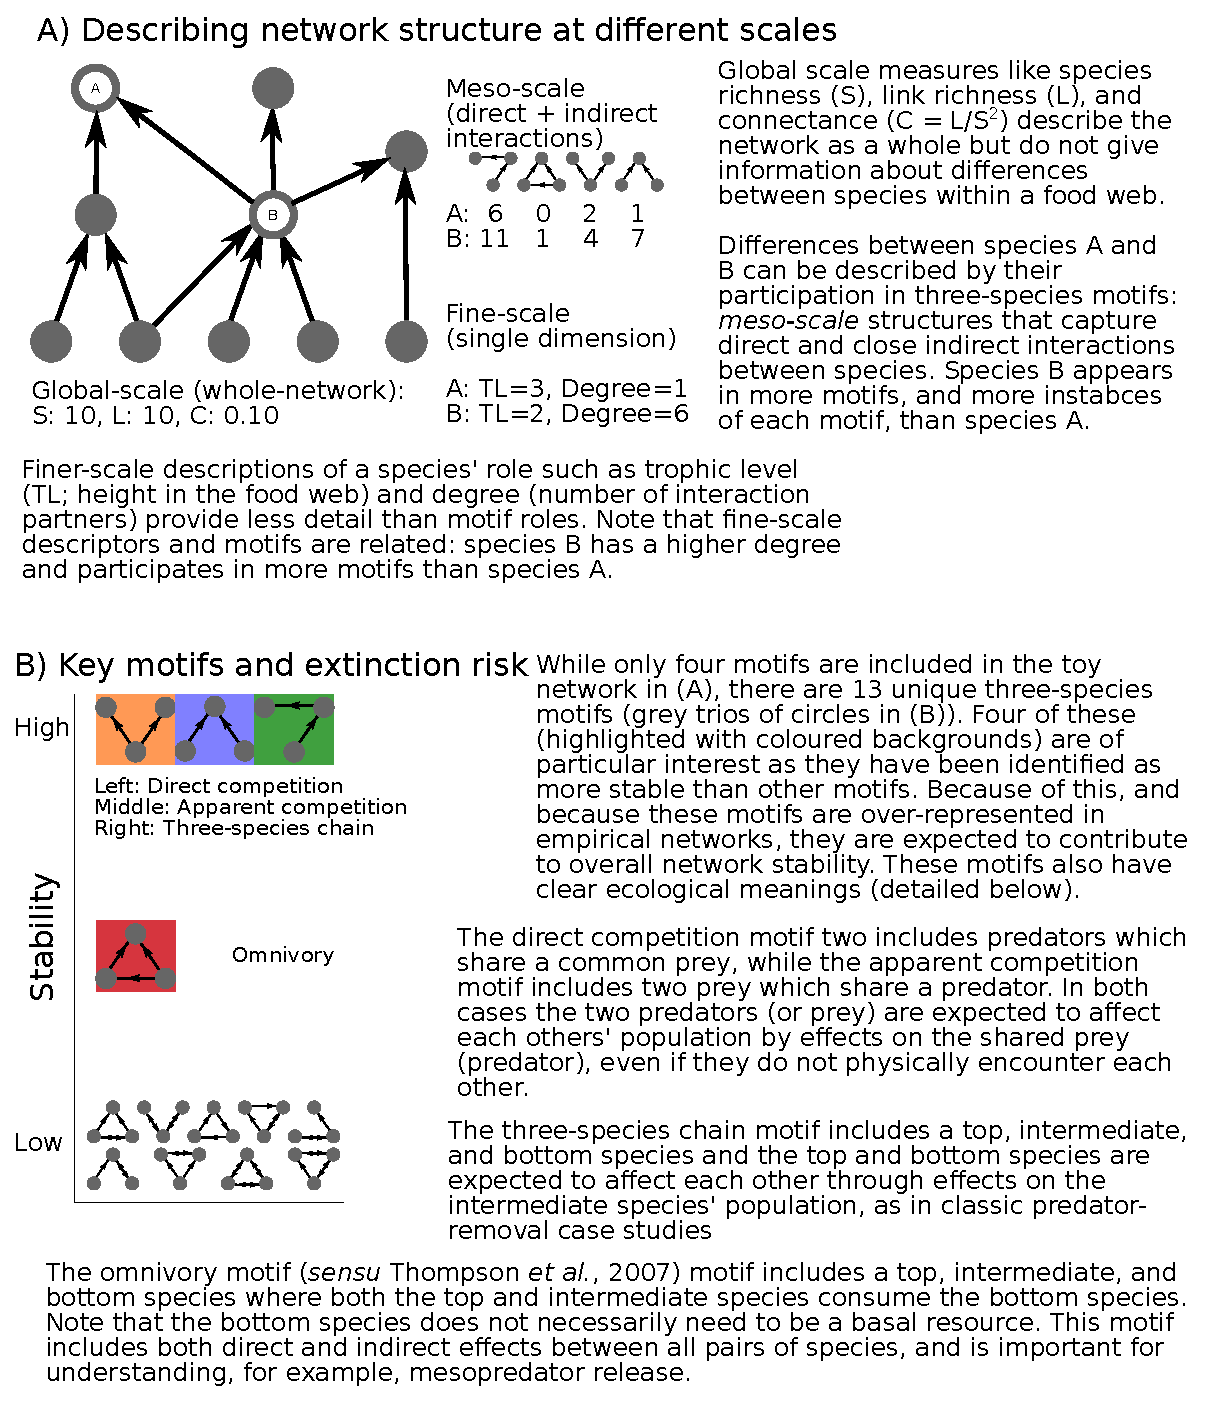
\includegraphics[width=.9\textwidth]{figures/motifs_box.eps}
        %DIF >  \textbf{Figure 1.} A brief introduction to motifs.
        %DIF >  \label{motifs}
    % \end{figure}

    %DIF <  \begin{figure}[h!]
  %DIF <    \caption{Here we show relationships between a species' position on the first three principal components axes and mean time to extinction. For interpretation of the axes, see Fig.~\ref{PCA_plots}.}
  %DIF <    \label{PCA_lmers}
  %DIF <    \includegraphics[height=0.75\textheight]{figures/extinction_order/PCA_position_lmer_summary_paper_full.eps}
  %DIF <    \end{figure}
%DIF >  \vspace{24pt}


%DIF <  \begin{figure}[h!]
  %DIF <    \caption{Here we show how the predicted time to extinciton in a linear model including fixed effects of role dissimilarity, path length, connectance, and their interaction varies over (\textbf{A}) role dissimilarity, and (\textbf{B}) path length. Line colours indicate connectance. We fit separate models for each level of species richness (50-100 species, in steps of 10). [[Consider adding some indication of significance.]]}
  %DIF <    \label{lmerfig}
  %DIF <    \includegraphics[height=.75\textheight]{figures/extinction_order/dissimilarity_fits_summary_paper_full.eps}
  %DIF <    \end{figure}
%DIF >  \end{spacing}


    \begin{figure}[ht!]
        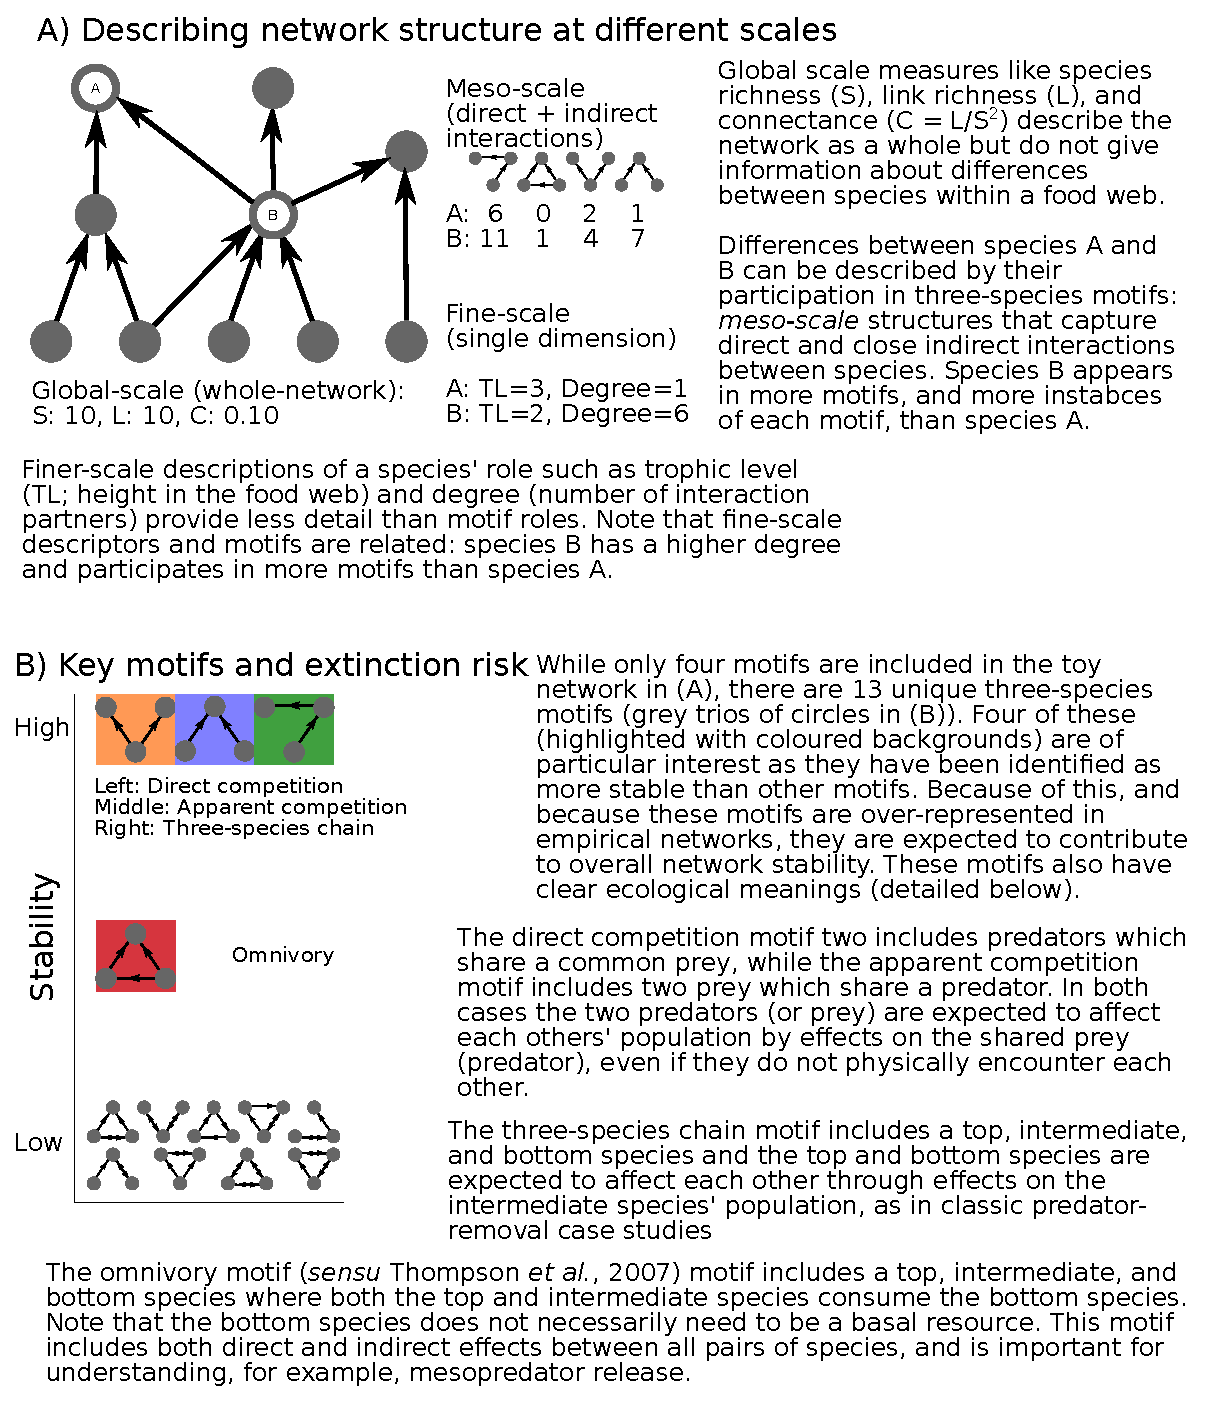
\includegraphics[width=.9\textwidth]{figures/motifs_box.eps}
        \caption{A brief introduction to motifs.}
        \label{motifs}
    \end{figure}

    \clearpage


\DIFaddbegin 
    \begin{figure}[ht!]
        \centering
        \includegraphics[width=\textwidth]{figures/roles/persistence_vs_positions_freq.eps}
        \caption{\DIFaddFL{Mean persistence time was significantly related to the frequency of appearing in different motif positions (R$^2$=0.081). The figure is based on the fixed effects in a regression of persistence against participation in positions in the apparent competition, direct competition, omnivory, three-species chain and motifs, with all positions in the `other' (loop-containing; not shown) motifs grouped, as well as random effects of global network structure and network ID. Top positions have prey but no predators within the motif, bottom positions have predators but no prey within the motif, and middle positions have both prey and predators within the motif. We show the marginal effects of increasing frequencies of each position. As position frequencies must sum to 1, we weighted participation in other motifs by their mean values.}}
        \label{fig:persistence_positions}
    \end{figure}

    \clearpage


    \begin{figure}[ht!]
        \centering
        \includegraphics[width=\textwidth]{figures/positions_vs_Deg_freq.eps}
        \caption{\DIFaddFL{The frequencies of the bottom position in the direct competition motif and the bottom and middle positions in the three-species chain decreased with increasing degree while the frequencies of the other positions in our focal motifs increased. Species-normalised (frequency) roles explained 62.9\% of variation in degree. We show the marginal effects of increasing frequencies of each position. As position frequencies must sum to 1, we weighted participation in other motifs by their mean values.}}
        \label{fig:positions_deg}
    \end{figure}

\clearpage

    \begin{figure}[ht!]
        \centering
        \includegraphics[width=\textwidth]{figures/roles/persistence_vs_degTL.eps}
        \caption{\DIFaddFL{Mean persistence time increased with increasing degree for species at low trophic levels (STL 1-2) but decreased with increasing degree for species at high trophic levels (STL \textgreater2). The figure is based on the fixed effects in a regression of persistence against degree, trophic level, their interaction, and a random effect of global network structure. We also give the marginal R$^2$ for the regression (fixed effects only).}}
        \label{fig:persistence_degTL}
    \end{figure}

\clearpage

%DIF >  \section*{Appendices}

%DIF >  \begin{spacing}{2.0}

%DIF >  All of the following Appendices are included as supplemental information:

    %DIF >  \subsection*{S1: Testing consistence of times to extinction}

    %DIF >      Supplemental methods and results related to testing whether the identity of the removed species has a large effect on the time to extinction for non-removed species. Includes \textbf{Figure S1}.

    %DIF >  \subsection*{S2: Details of PERMANOVA results}

    %DIF >      Supplemental results for PERMANOVAs testing whether species' overall roles are related to their mean times to exinction. Includes \textbf{Figure S2, Tables S1-S2}.

    %DIF >  \subsection*{S3: Relating motifs roles to other measures}

    %DIF >      Gives the slopes of relationships between motif roles and degree or shortest trophic level (STL) in \textbf{Tables S3-S4}.

    %DIF >  \subsection*{S4: Motif labels}

    %DIF >      \textbf{Figure S3} illustrates the 13 unique three-species motifs and labels each one according to the naming scheme in~\citet{Stouffer2007}.

%DIF >  \end{spacing}
\DIFaddend 

\end{document}



